After looking at the unblinded data, an excess well compatible with 
$\mHi = 125~\GeV$ is observed. Nevertheless, there is also an excess in the low 
dilepton mass region with $\mt \sim 130-160~\GeV$, which is not likely to be from 
the low mass Higgs hypothesis. The $\mt$ distributions in the 0-jet bin 
and 1-jet bin for events with $\mll<80~\GeV$ are shown in Fig.~\ref{fig:histo_mt_0j_hw160}. 
We have studied the two-dimensional analysis in detail by looking at several 
$H(125) \to \W\W$ free regions to check if there is any particular feature in the data. 
These four analyses have been performed, keeping the rest of the analysis chain unchanged:

\begin{itemize}
  \item[(1)] excluding events if $m_{T} < 130~\GeV$ and $\mll < 60~\GeV$, this rejects Higgs 
  events with $\mHi = 125~\GeV$, with reasonable performance at higher masses;
  \item[(2)] performing the analysis on top-tagged events;
  \item[(3)] performing the analysis on same-sign lepton pair events;
  \item[(4)] performing the analysis using H(125) as part of the background.
\end{itemize}

\begin{figure}[hbt!]
\begin{center}
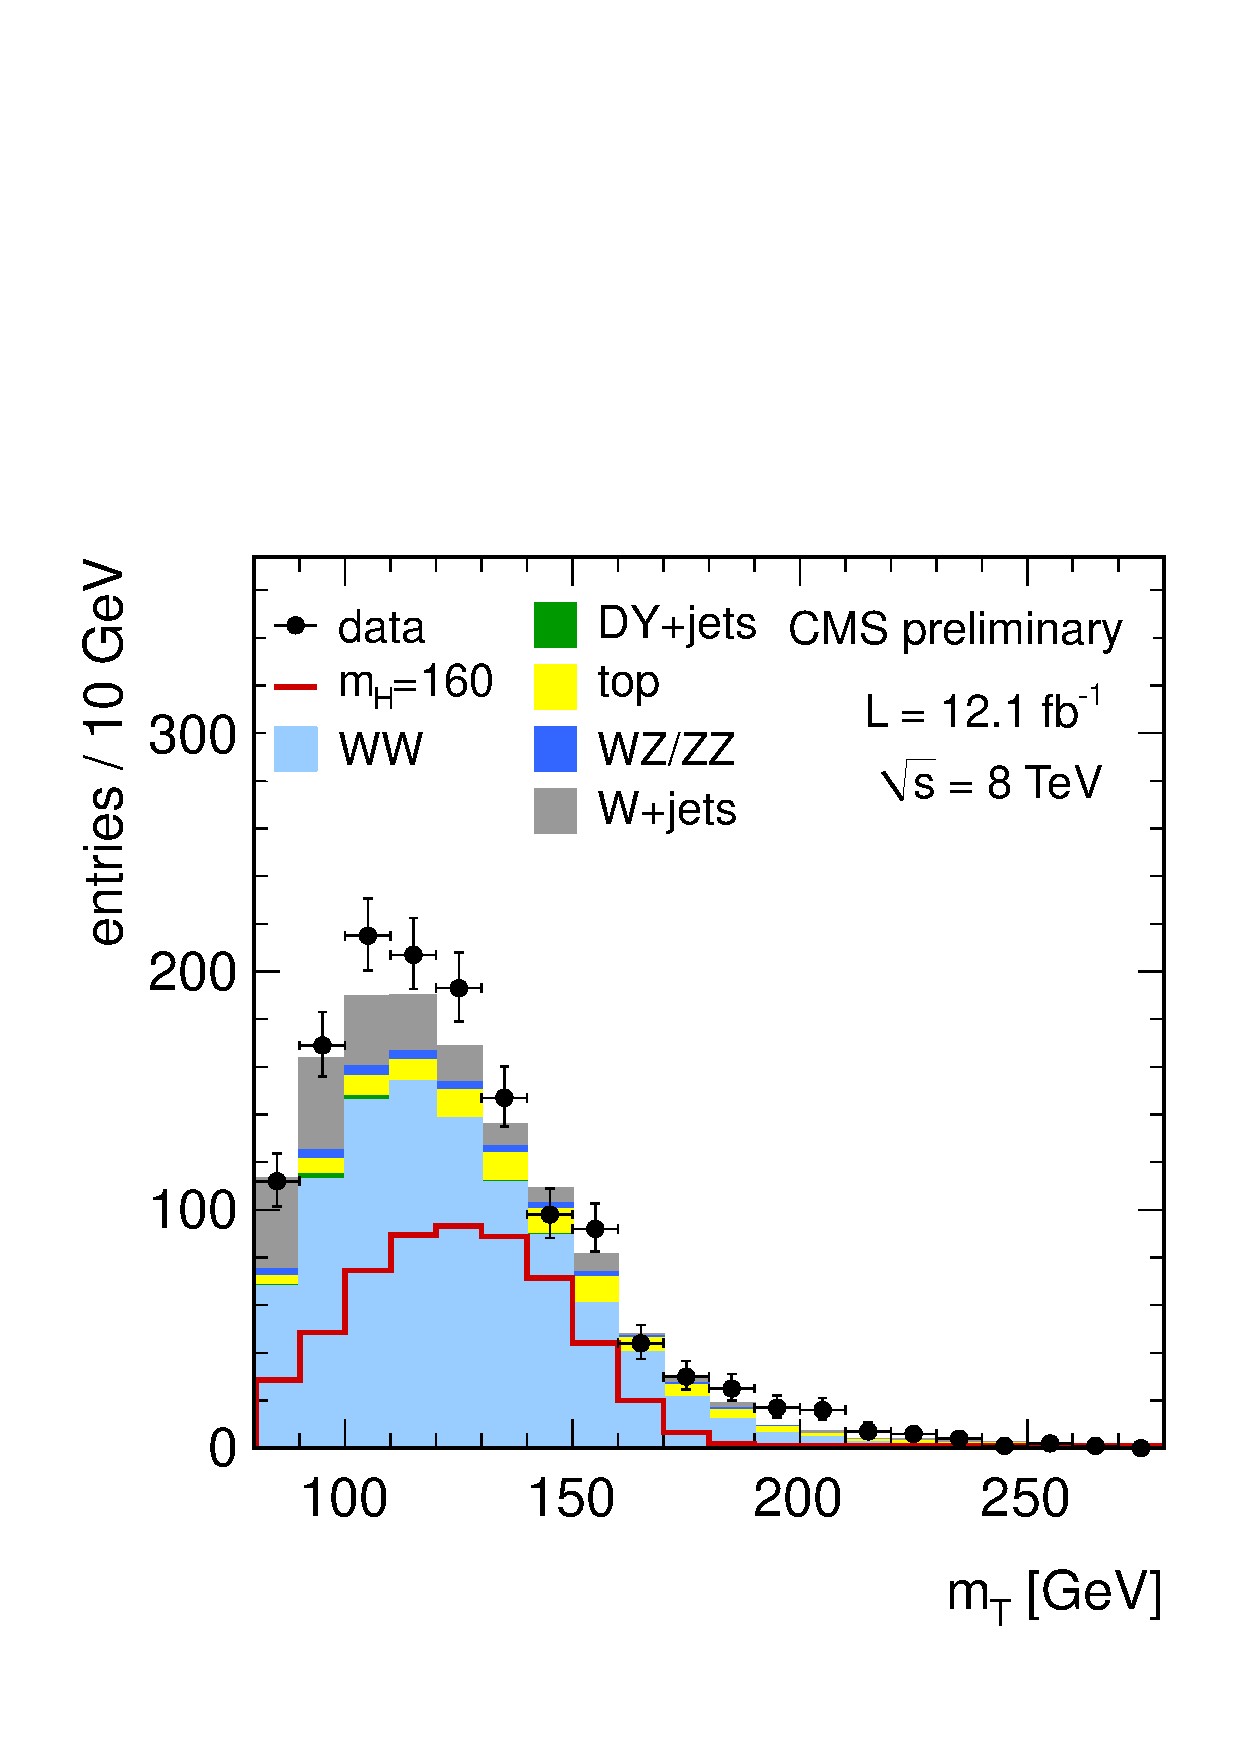
\includegraphics[width=0.49\linewidth]{figures/histo_mt_0j_hw160.pdf}
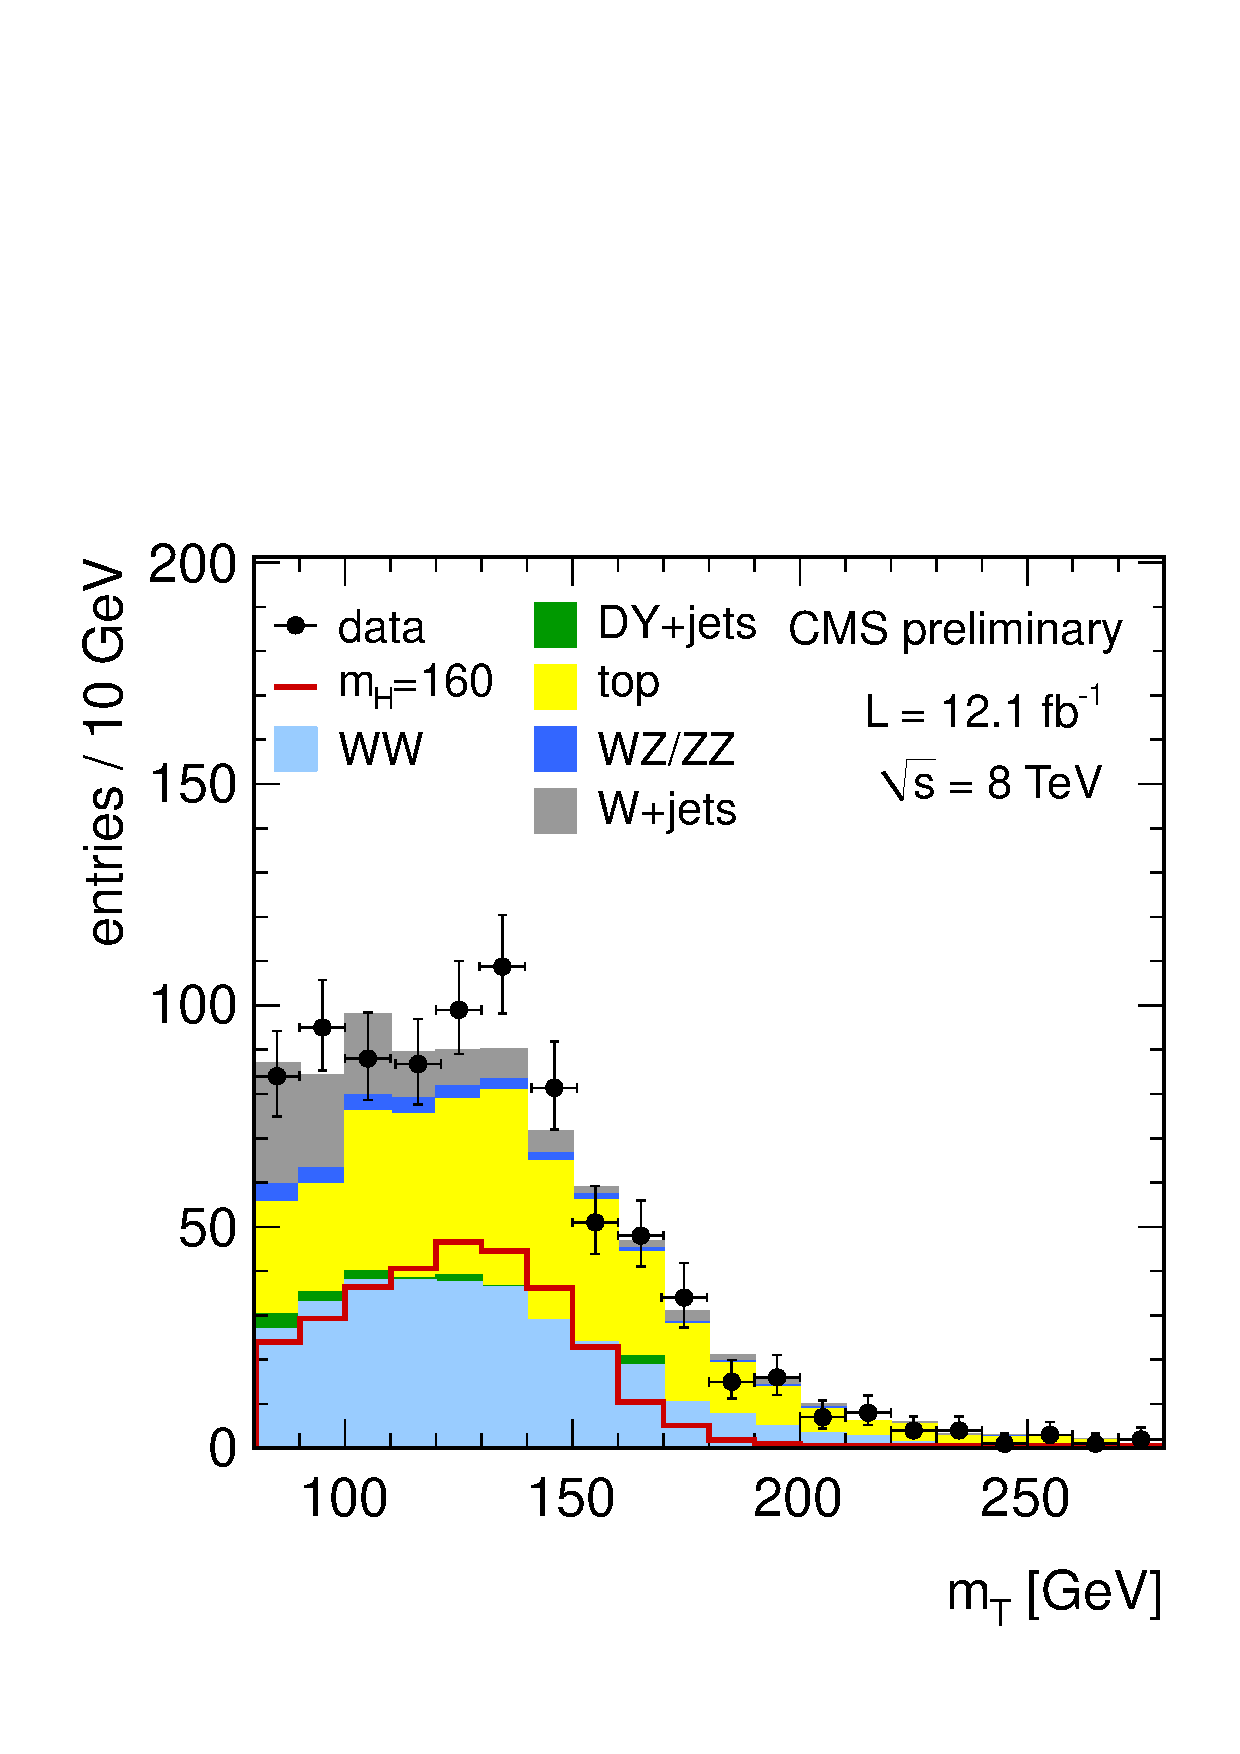
\includegraphics[width=0.49\linewidth]{figures/histo_mt_1j_hw160.pdf}
\caption{\label{fig:histo_mt_0j_hw160}\protect $\mt$ distributions in the 0-jet bin (left) 
and 1-jet bin (right) for events with $\mll<80~\GeV$.}
\end{center}
\end{figure}

\subsection{Excluding Events with $m_{T} < 130~\GeV$ and $\mll < 60~\GeV$}
This analysis excludes events with $m_{T} < 130~\GeV$ and $\mll < 60~\GeV$, i.e. the preferred 
region for $\mHi = 125~\GeV$. The Expected and observed limits for the two-dimensional analysis 
are shown in Fig.~\ref{fig:limits8TeV_ofshapeN_HCP_2D_NoH125}, while the expected and observed 
significances are shown in Fig.~\ref{fig:significance8TeV_ofshapeN_HCP_2D_NoH125}.

\begin{figure}[hbt!]
\begin{center}
  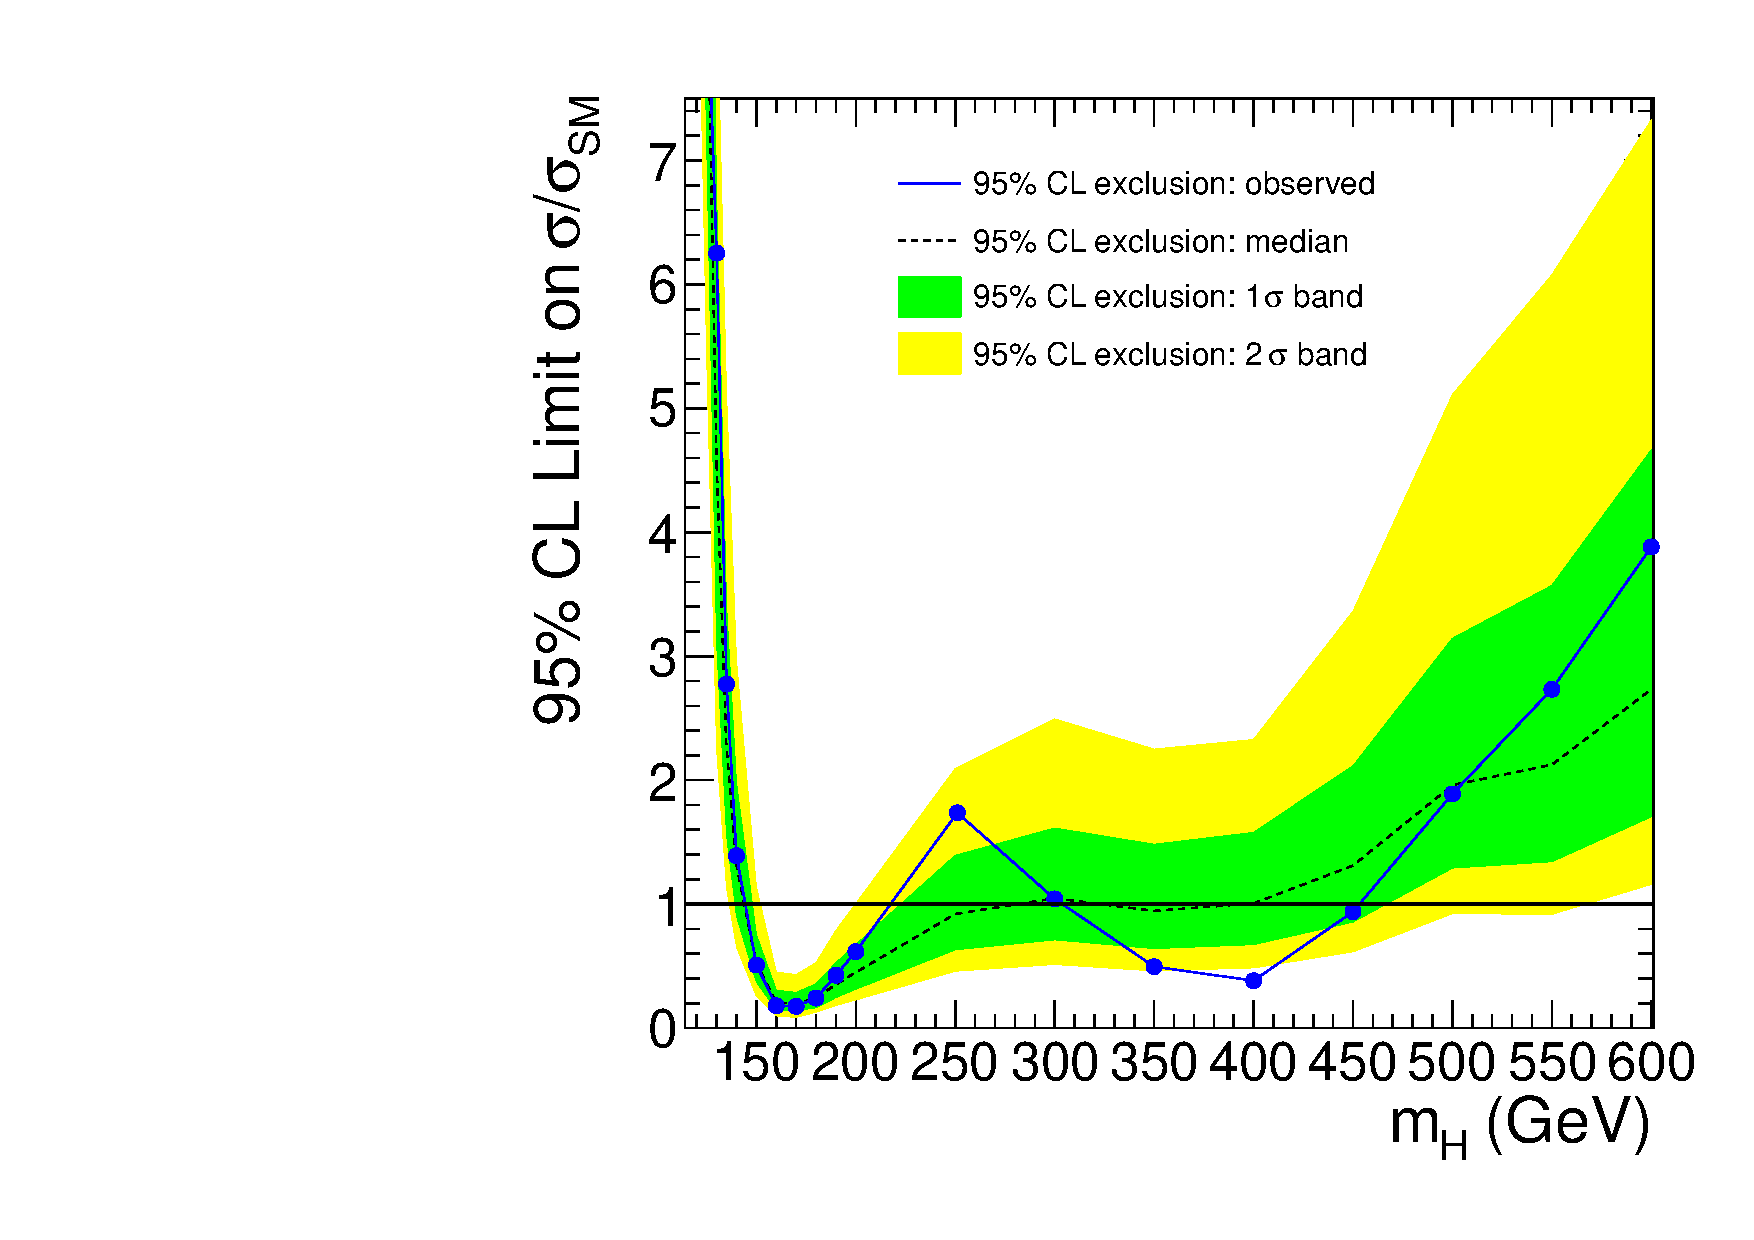
\includegraphics[width=0.49\textwidth]{figures/limits8TeV_ofshape0_HCP_2D_NoH125.pdf}
  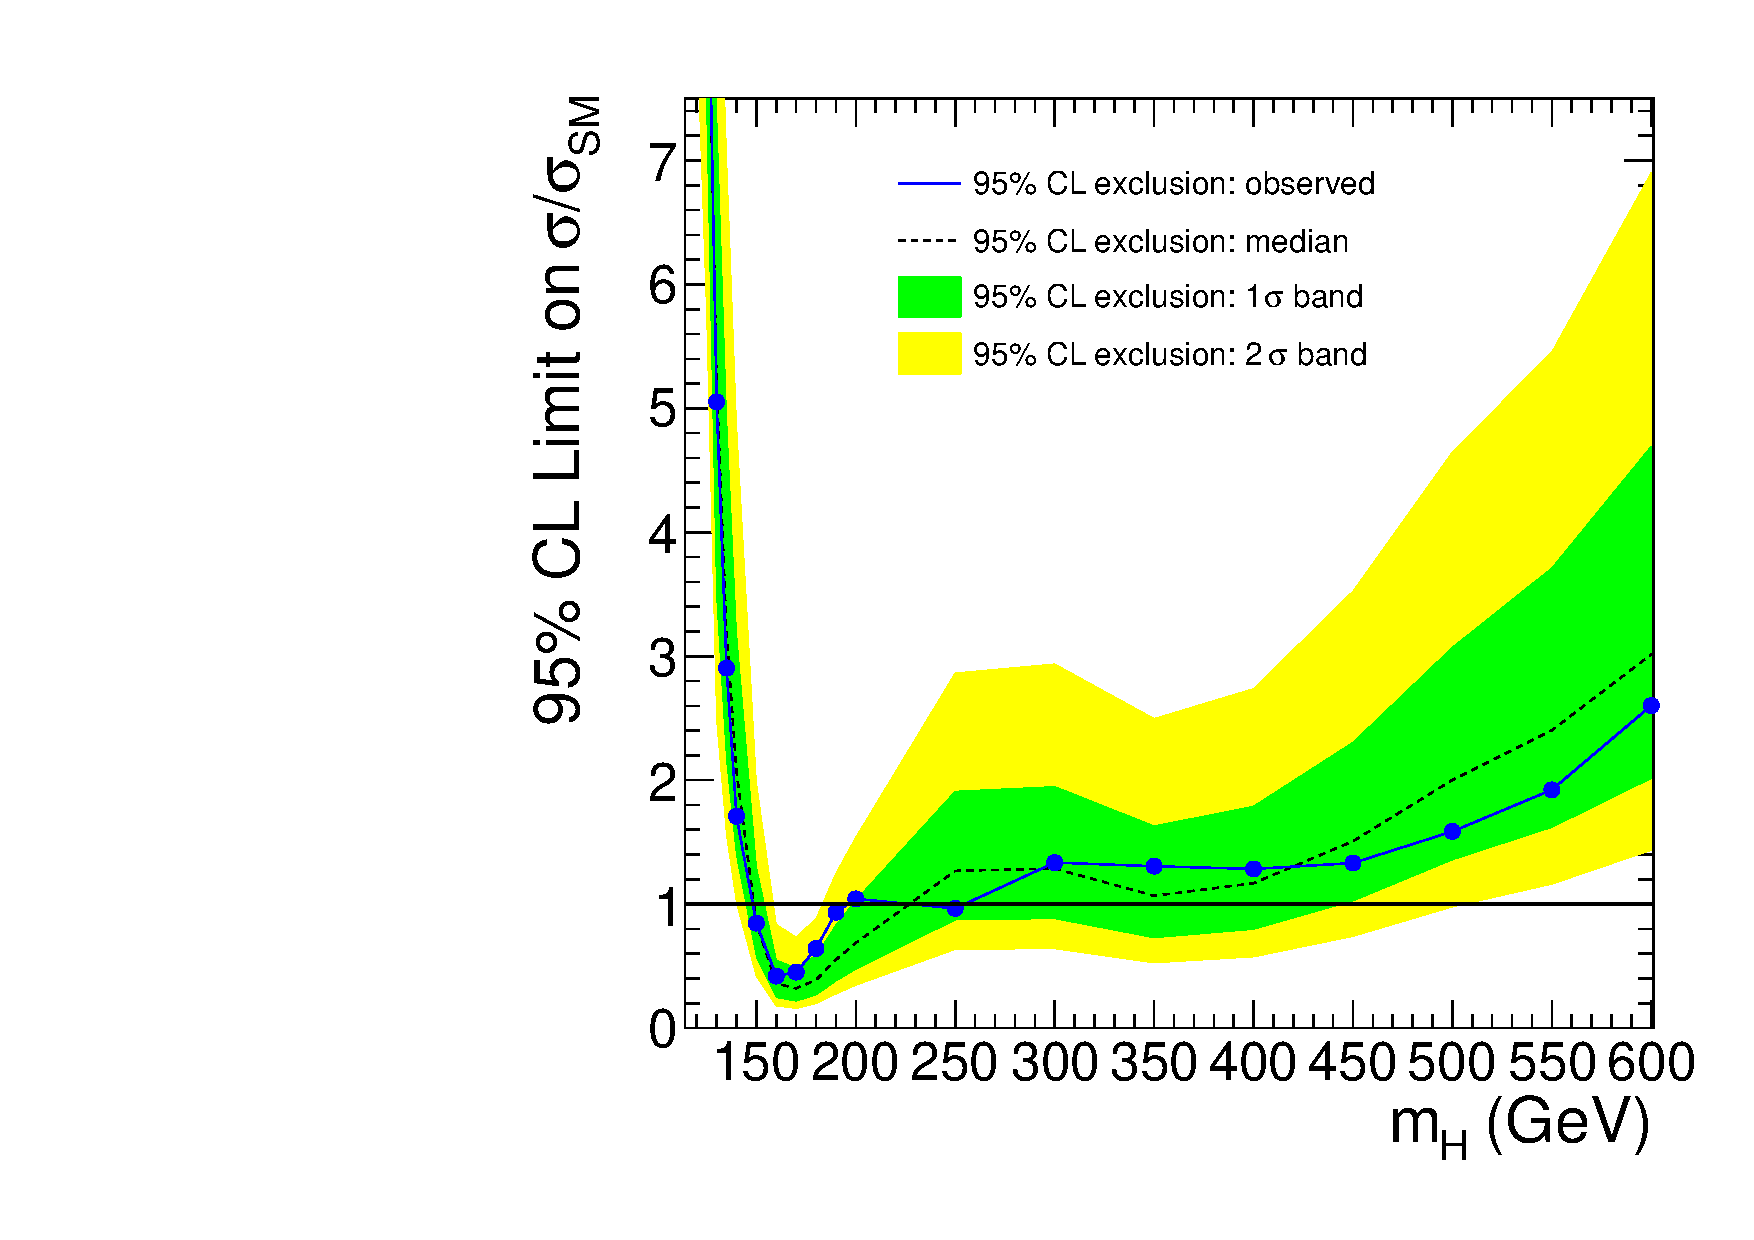
\includegraphics[width=0.49\textwidth]{figures/limits8TeV_ofshape1_HCP_2D_NoH125.pdf}
  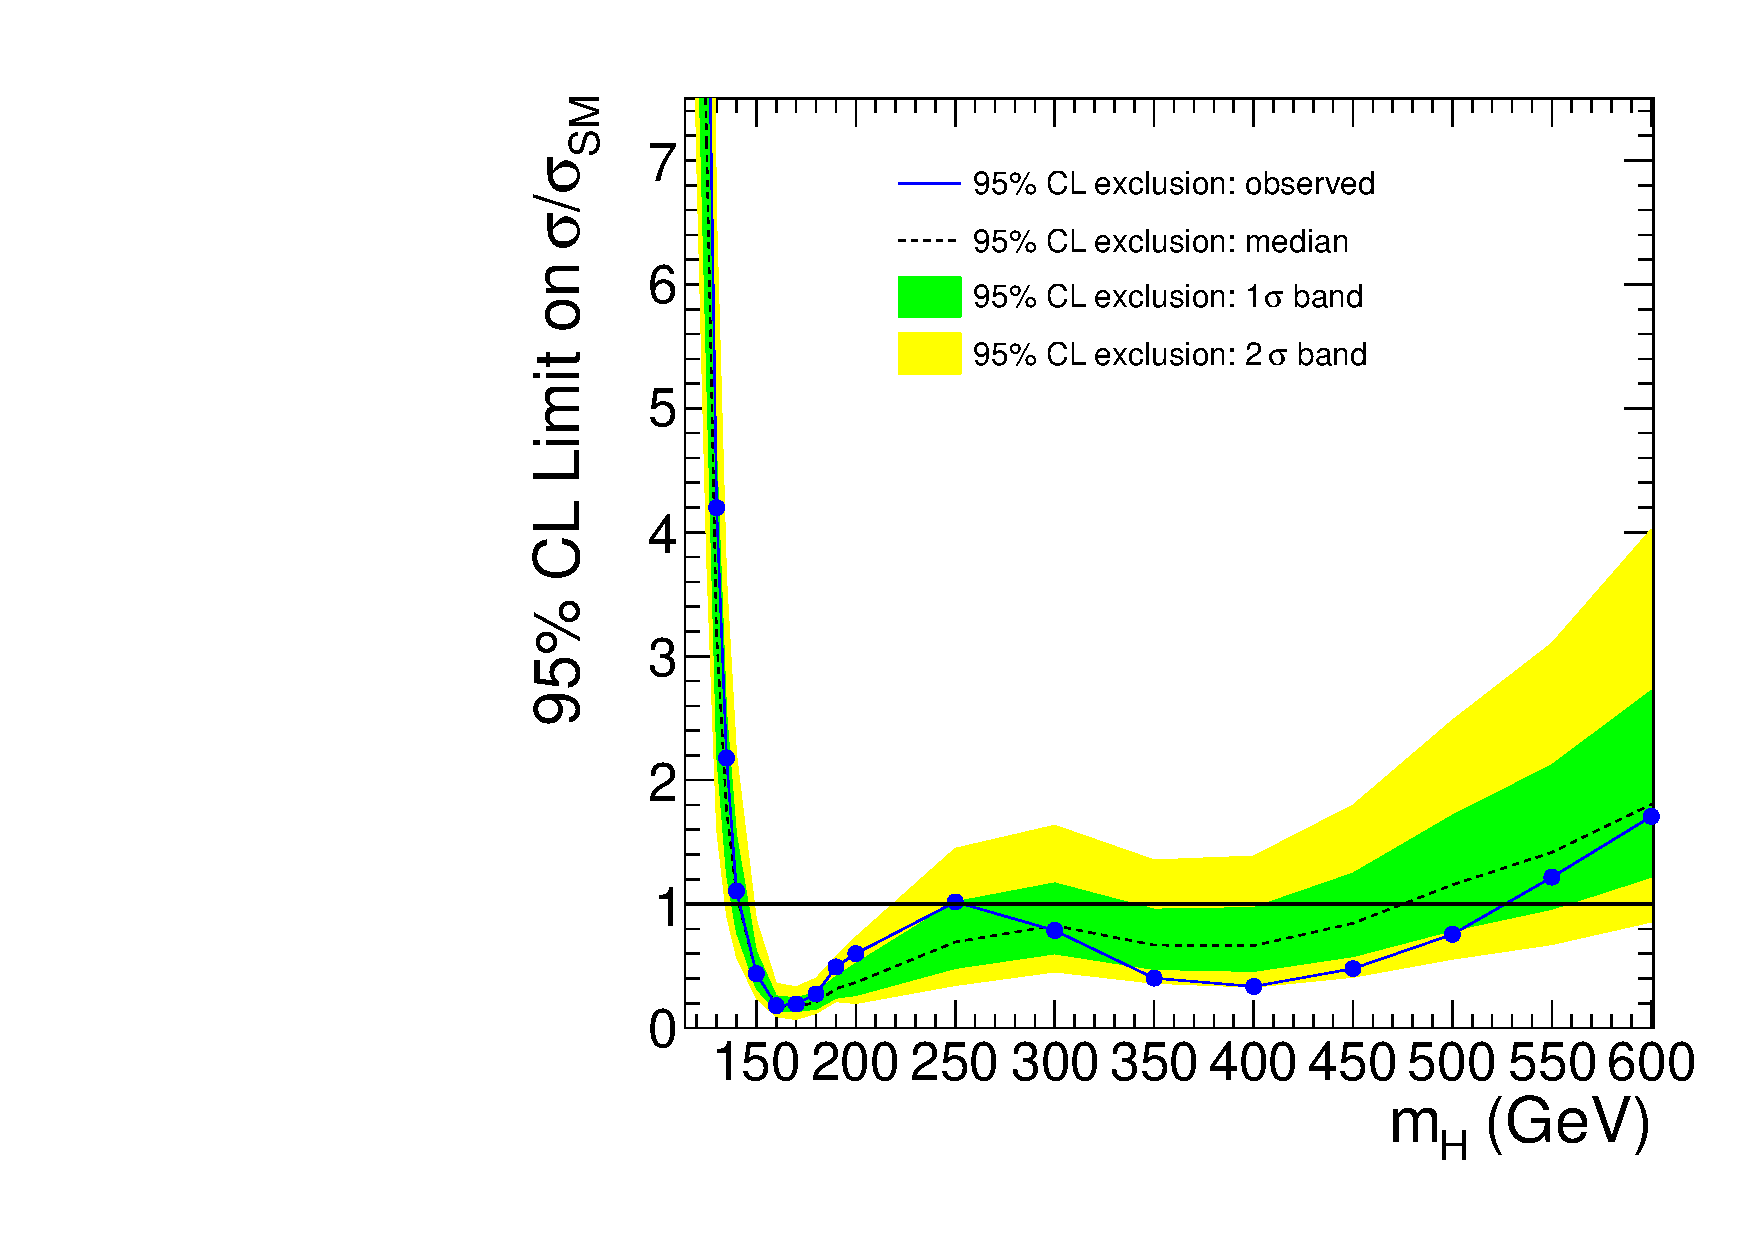
\includegraphics[width=0.49\textwidth]{figures/limits8TeV_ofshape_HCP_2D_NoH125.pdf}
\caption{\label{fig:limits8TeV_ofshapeN_HCP_2D_NoH125}\protect Expected and observed limits for the two-dimensional 
analysis in the 0-jet bin (top left), 1-jet bin (top right), and 0/1-jet bins (bottom), for 
the analysis excluding events in the preferred H(125) region.}
\end{center}
\end{figure}

\begin{figure}[hbt!]
\begin{center}
  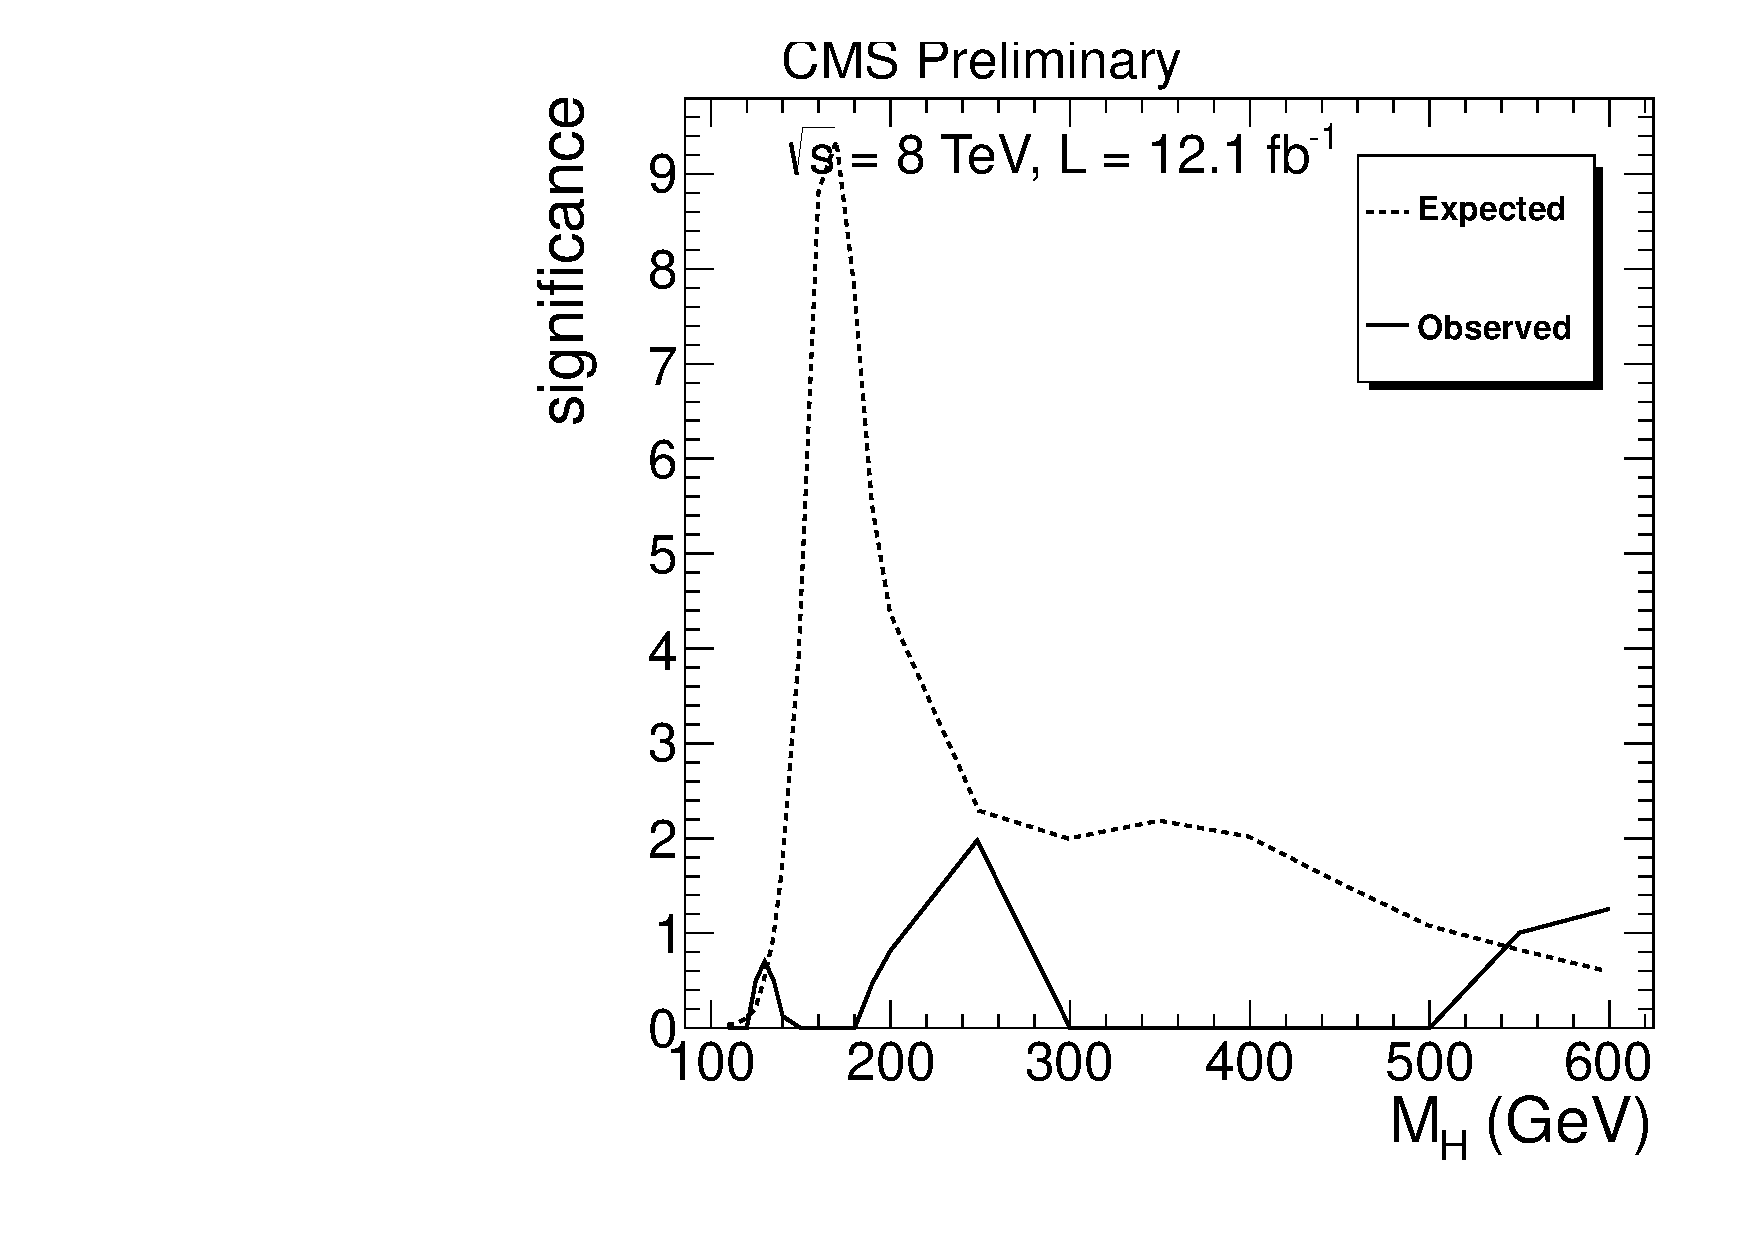
\includegraphics[width=0.49\textwidth]{figures/significance8TeV_ofshape0_HCP_2D_NoH125.pdf}
  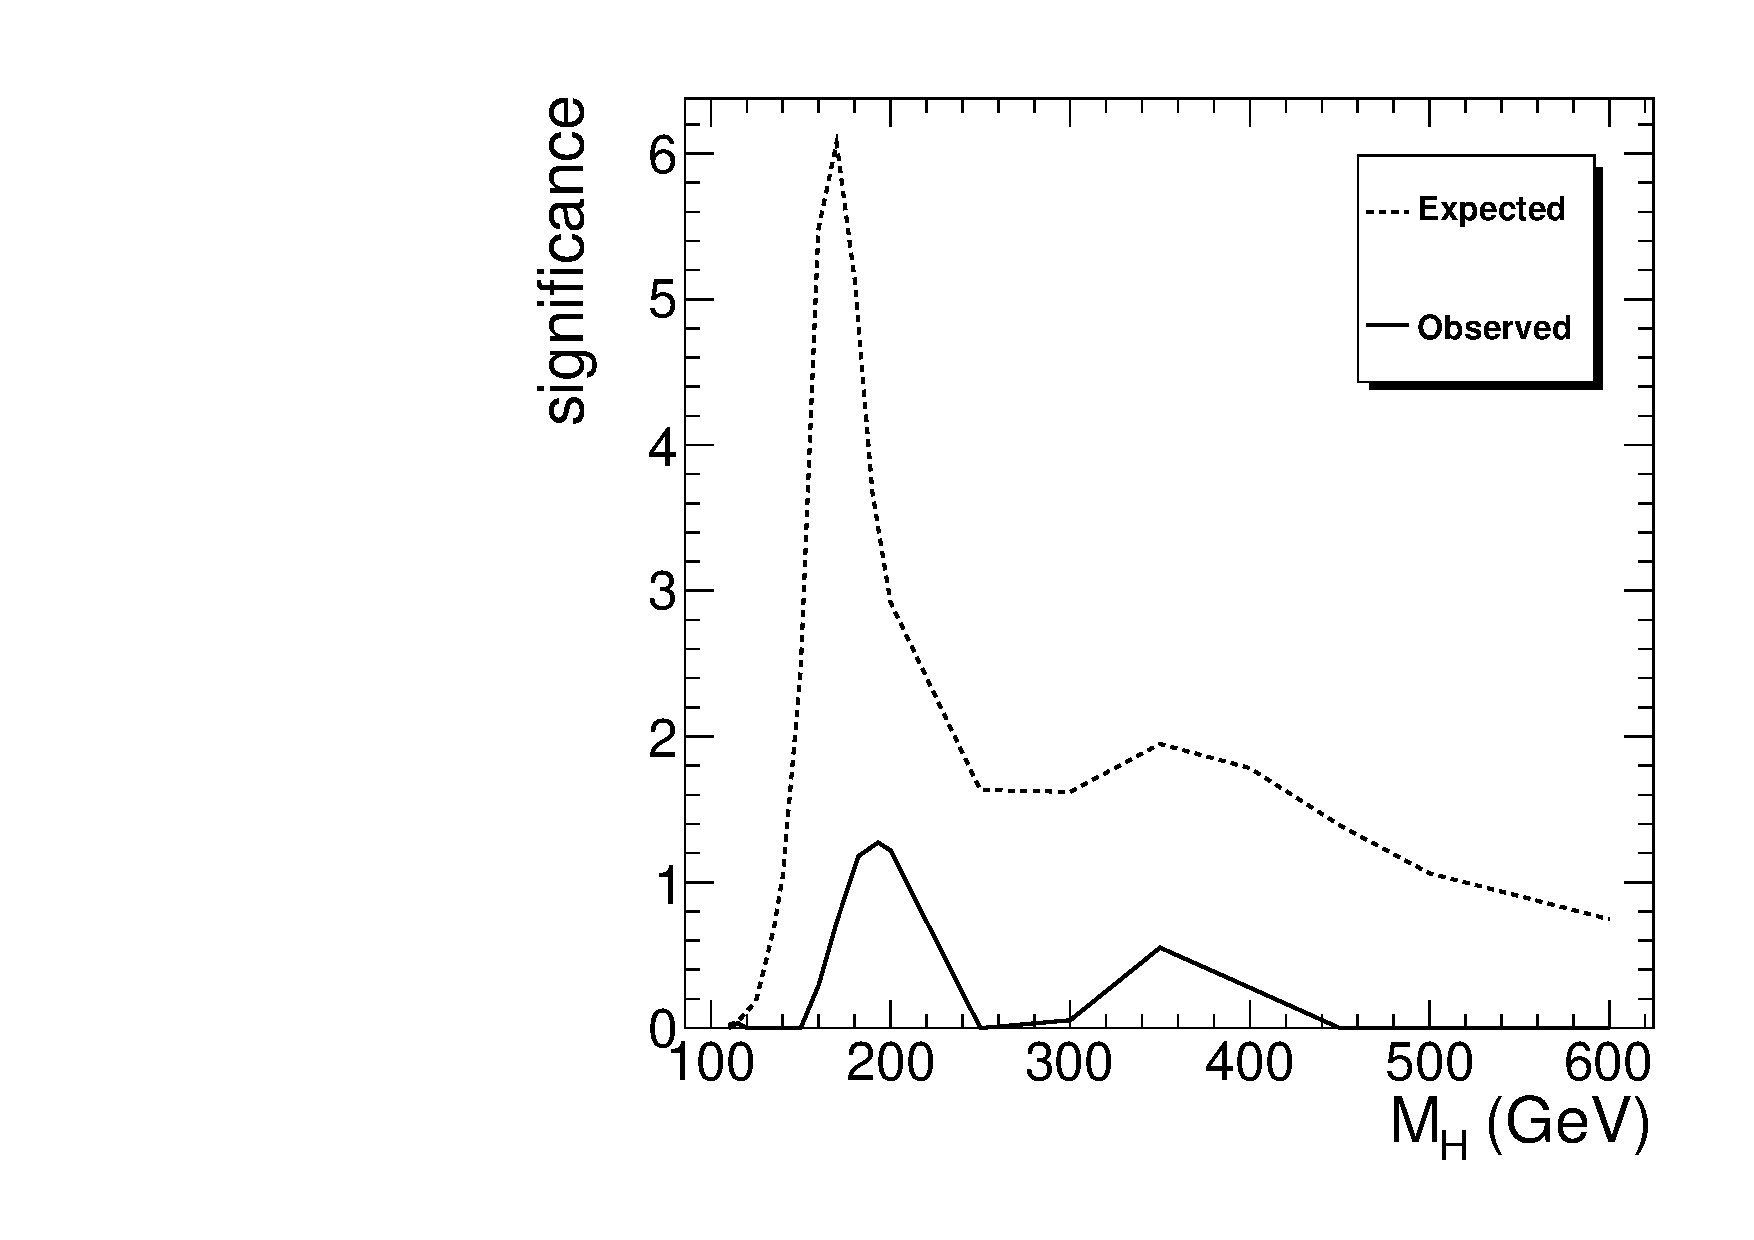
\includegraphics[width=0.49\textwidth]{figures/significance8TeV_ofshape1_HCP_2D_NoH125.pdf}
  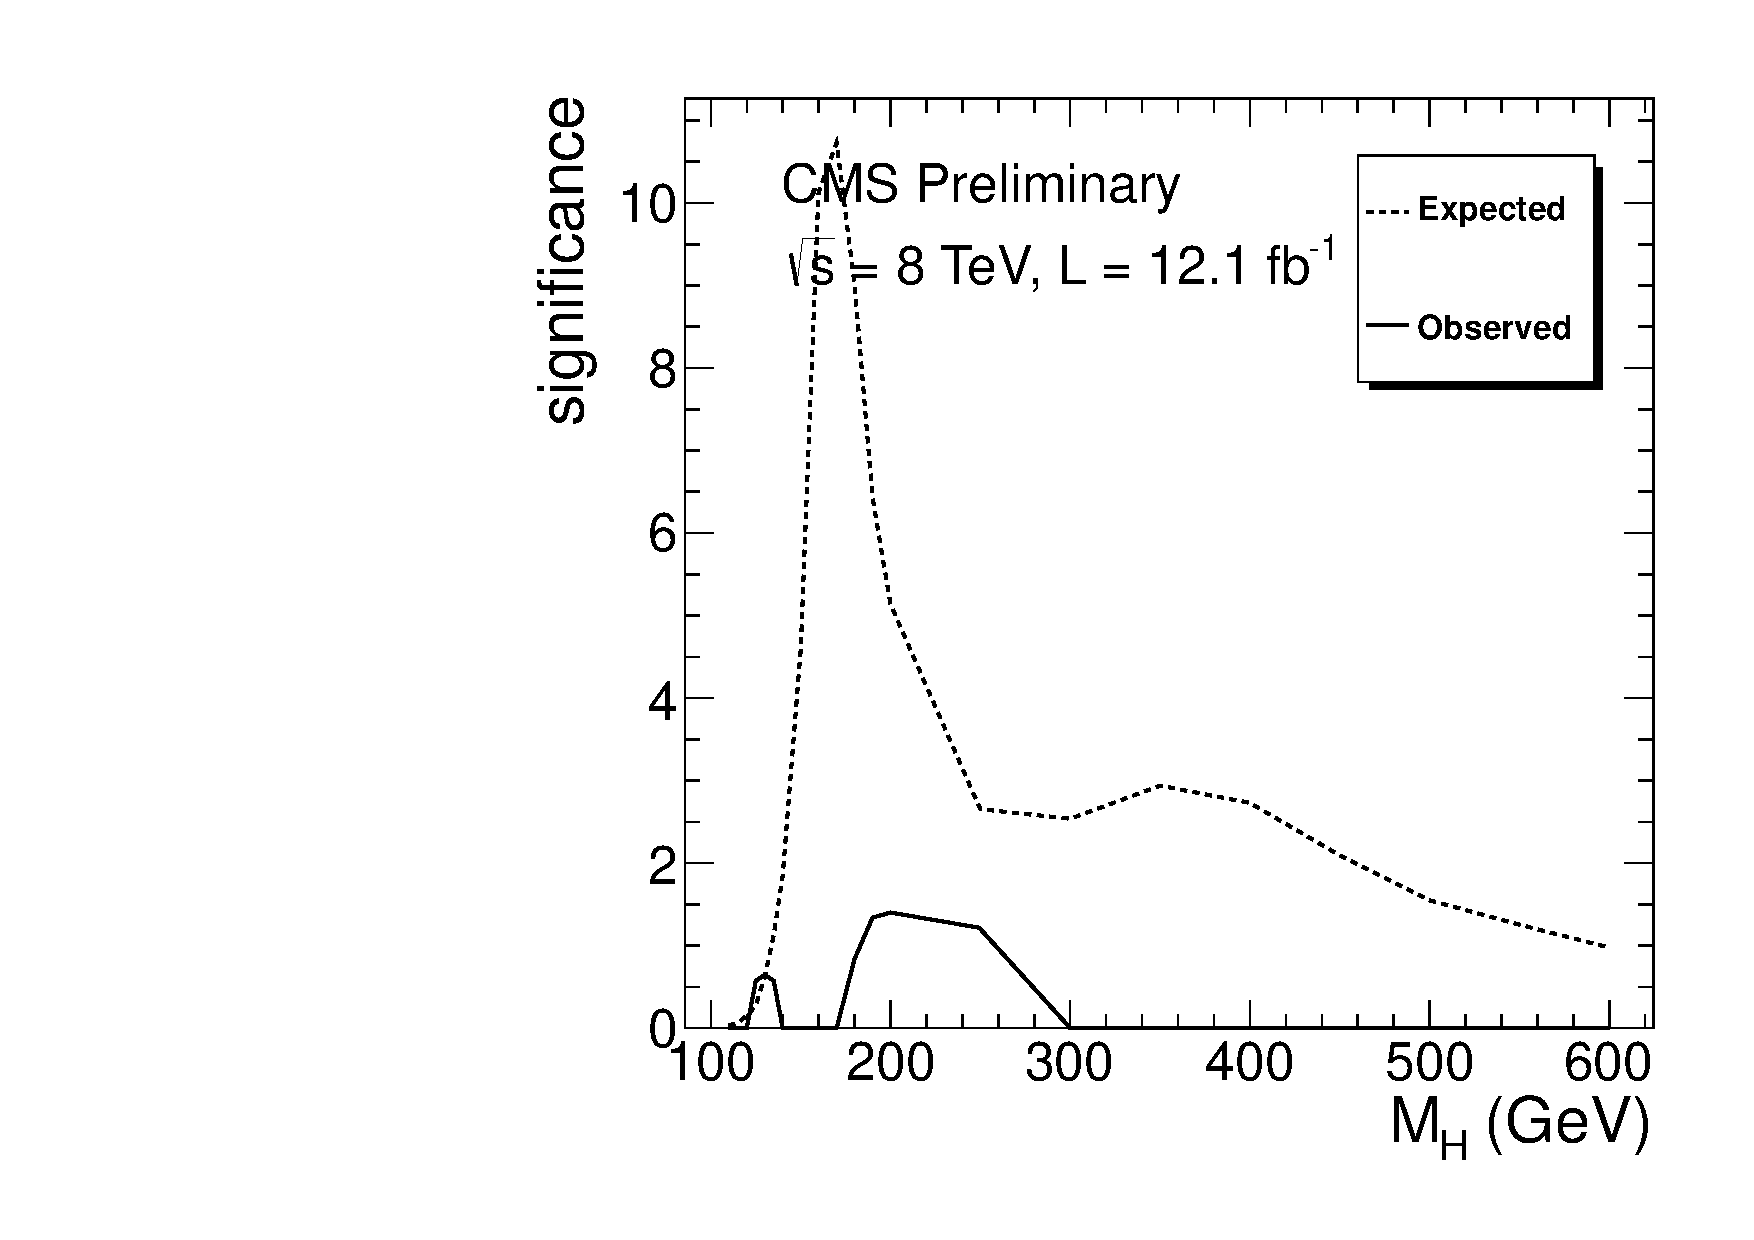
\includegraphics[width=0.49\textwidth]{figures/significance8TeV_ofshape_HCP_2D_NoH125.pdf}
\caption{\label{fig:significance8TeV_ofshapeN_HCP_2D_NoH125}\protect Expected and observed significance for the two-dimensional 
analysis in the 0-jet bin (top left), 1-jet bin (top right), and 0/1-jet bins (bottom), for 
the analysis excluding events in the preferred H(125) region.}
\end{center}
\end{figure}

\subsection{B-Tagged Region}
This analysis selects b-tagged events, i.e. it is enriched in top events, in particular in the 
1-jet bin. The $\mt$ distributions for events with $\mll<80~\GeV$ are shown in 
Fig.~\ref{fig:histo_mt_0j_hw160_btag}. The performance of this analysis is small due to the low 
rate of b-tagged Higgs events, although it is still reasonable. The Expected and observed limits for 
the two-dimensional analysis are shown in Fig.~\ref{fig:limits8TeV_ofshapeN_HCP_2D_BTAG}, while the expected and observed 
significances are shown in Fig.~\ref{fig:significance8TeV_ofshapeN_HCP_2D_BTAG}.

\begin{figure}[hbt!]
\begin{center}
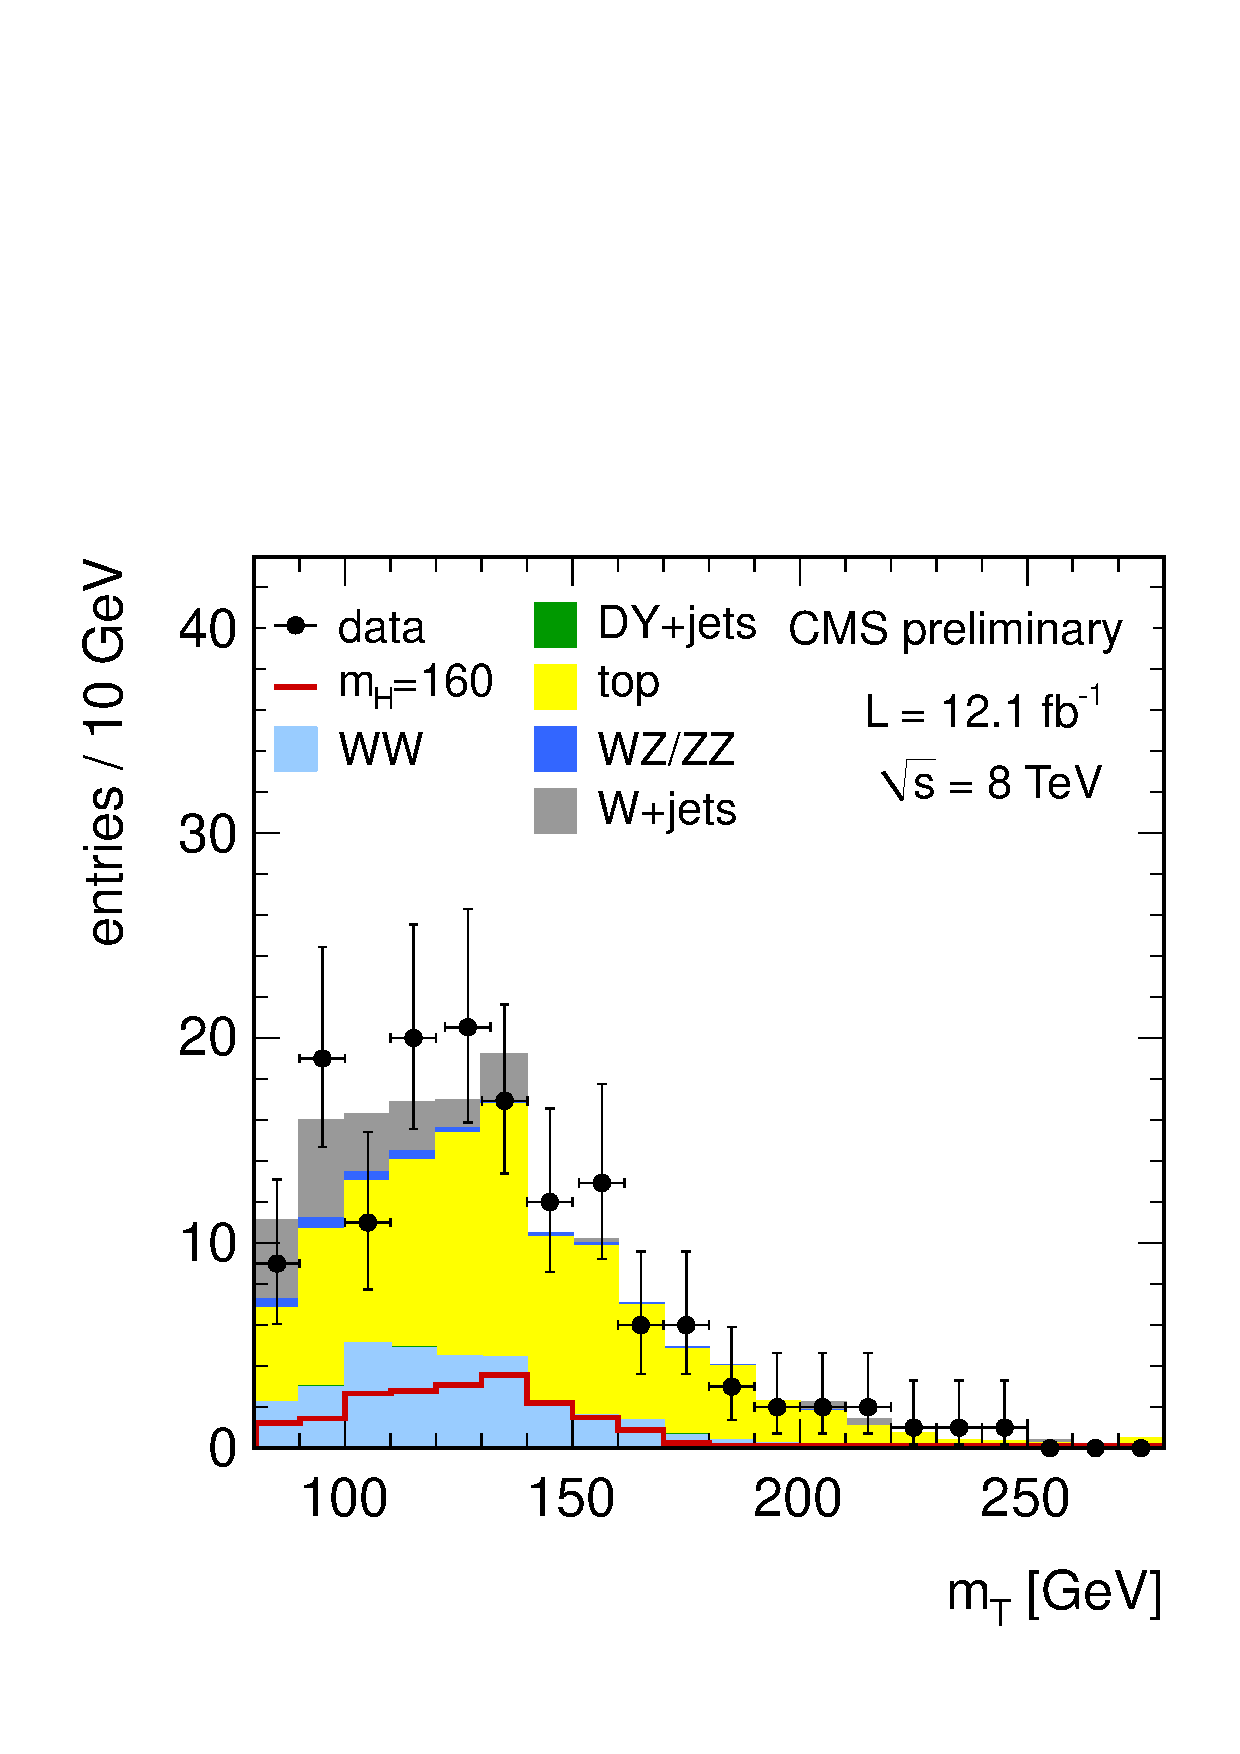
\includegraphics[width=0.49\linewidth]{figures/histo_mt_0j_hw160_btag.pdf}
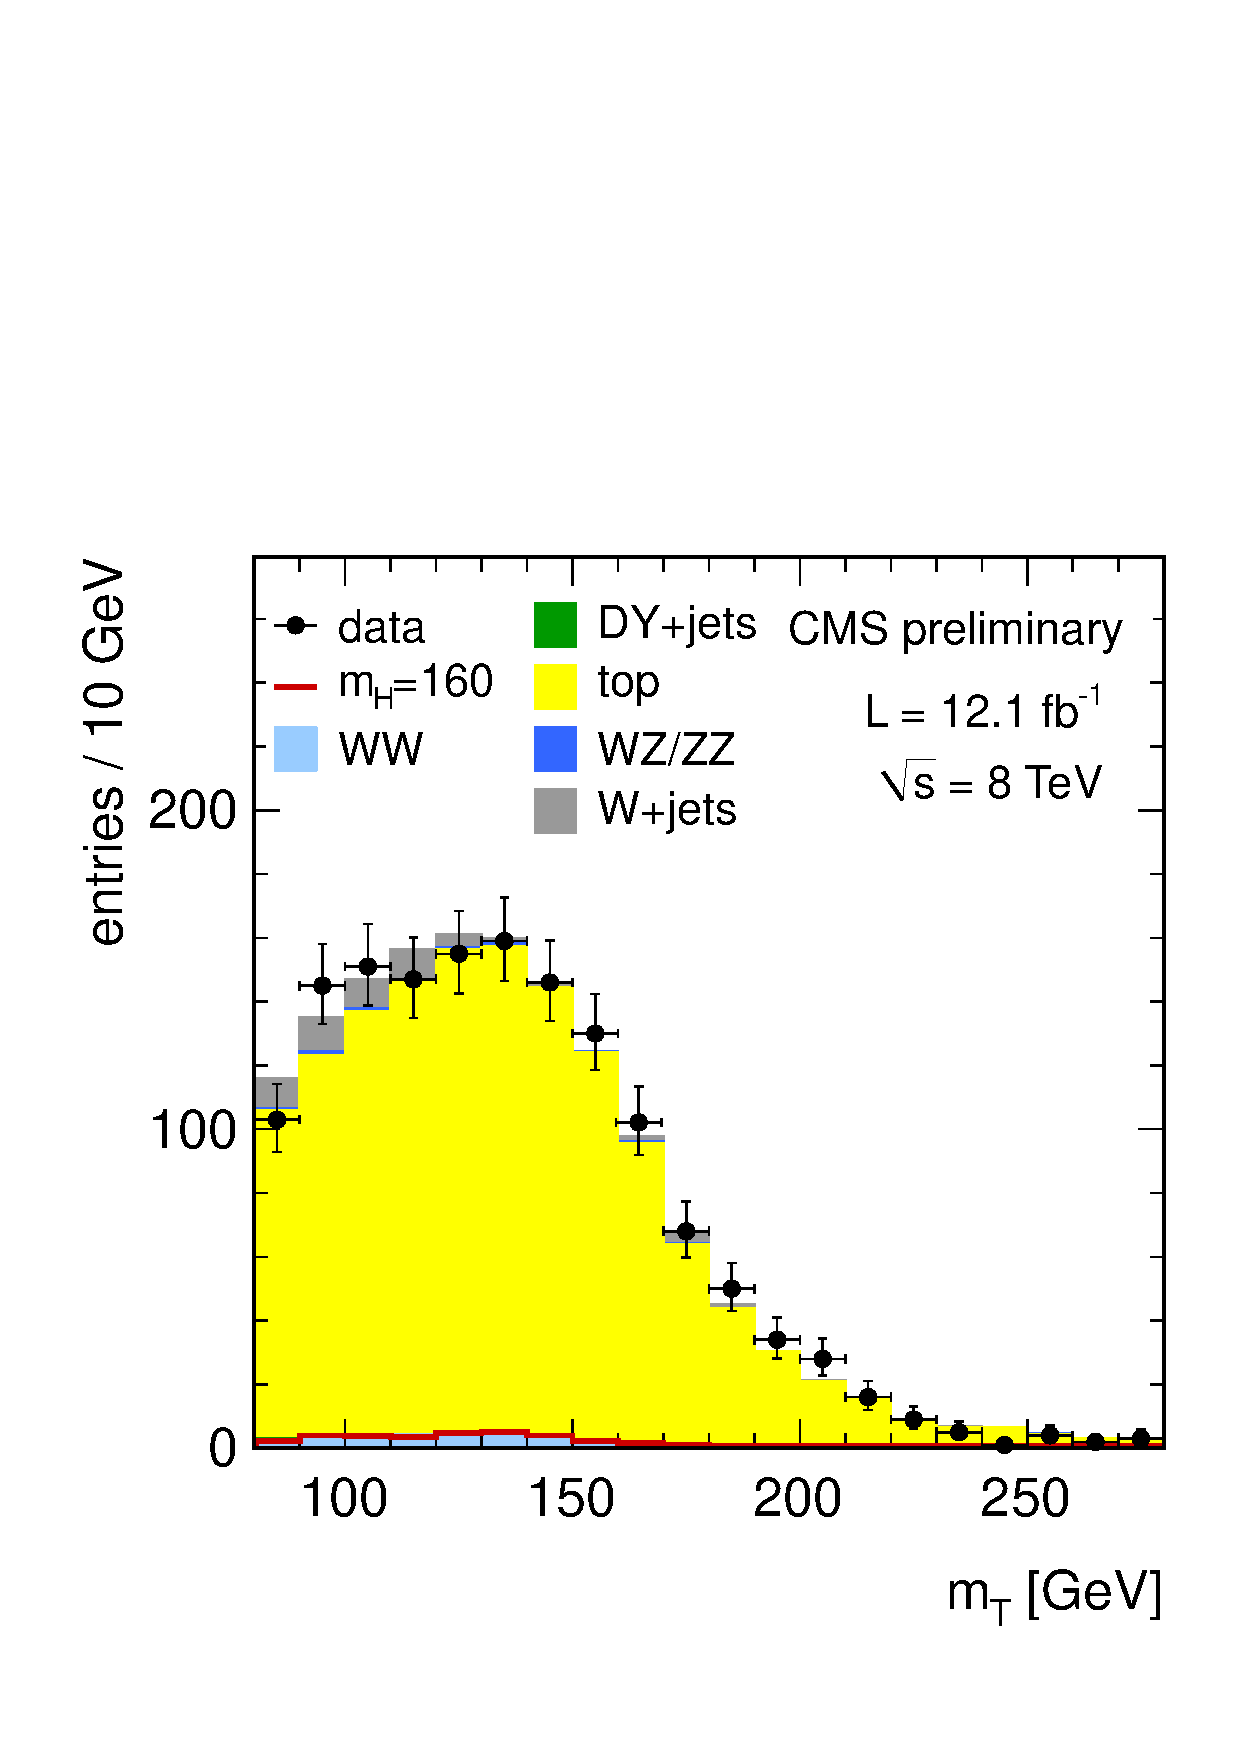
\includegraphics[width=0.49\linewidth]{figures/histo_mt_1j_hw160_btag.pdf}
\caption{\label{fig:histo_mt_0j_hw160_btag}\protect $\mt$ distributions in the 0-jet bin (left) 
and 1-jet bin (right) for events with $\mll<80~\GeV$ in the b-tagged region.}
\end{center}
\end{figure}

\begin{figure}[hbt!]
\begin{center}
  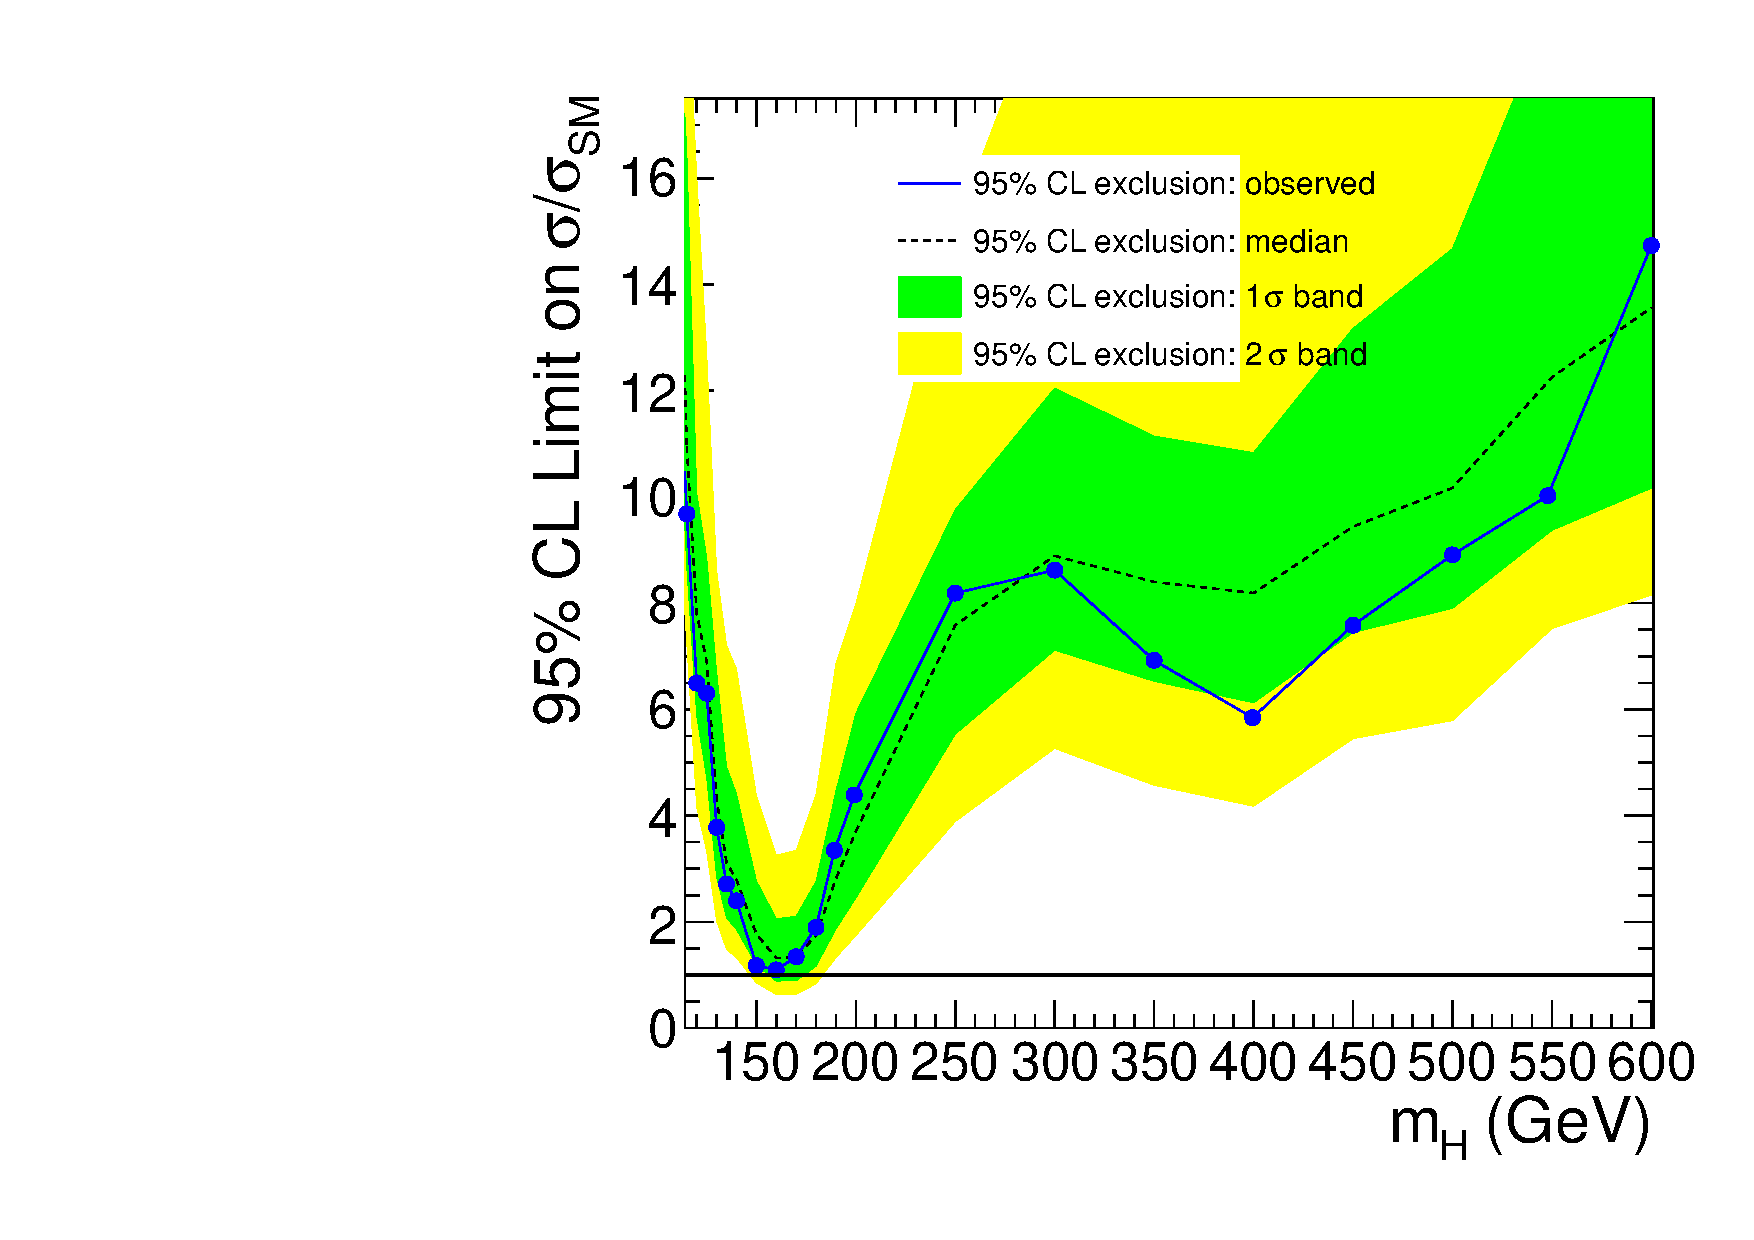
\includegraphics[width=0.49\textwidth]{figures/limits8TeV_ofshape0_HCP_2D_BTAG.pdf}
  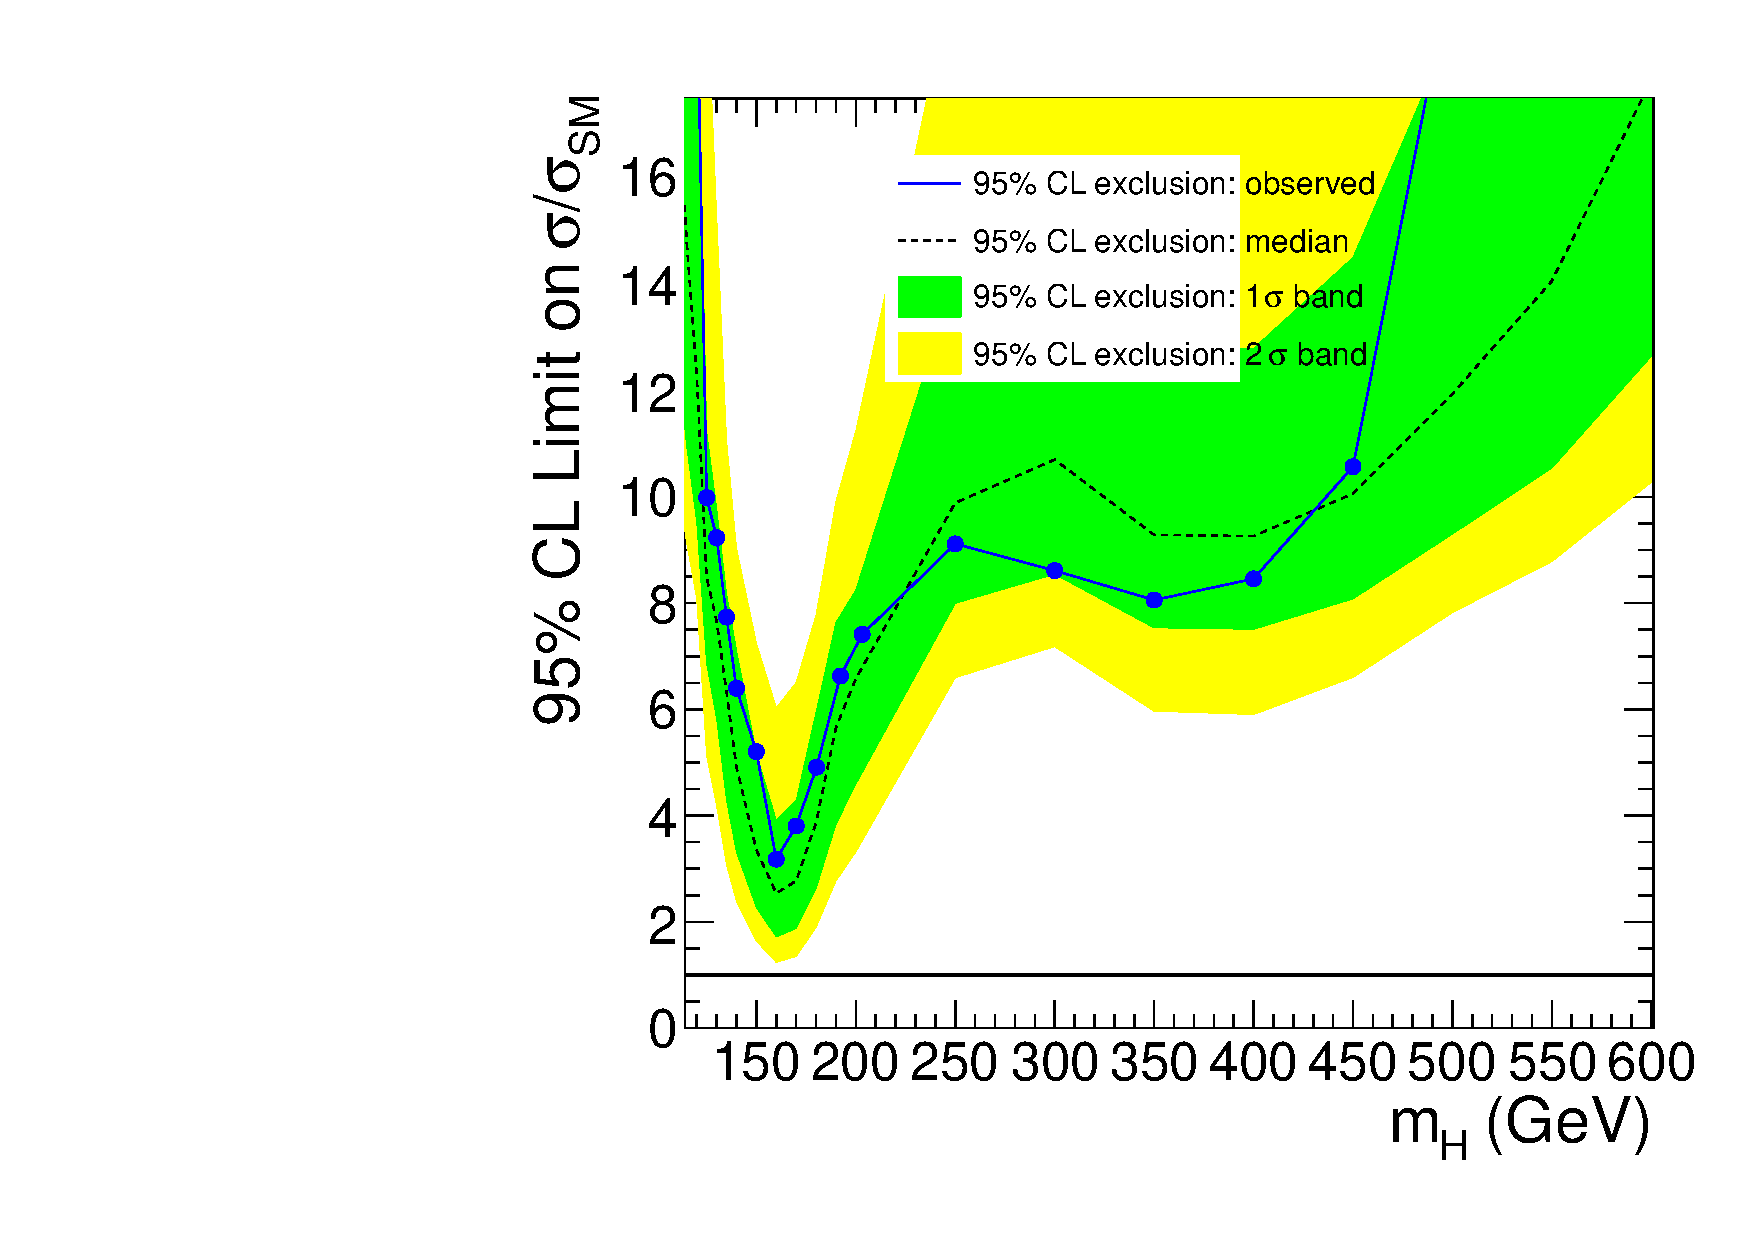
\includegraphics[width=0.49\textwidth]{figures/limits8TeV_ofshape1_HCP_2D_BTAG.pdf}
  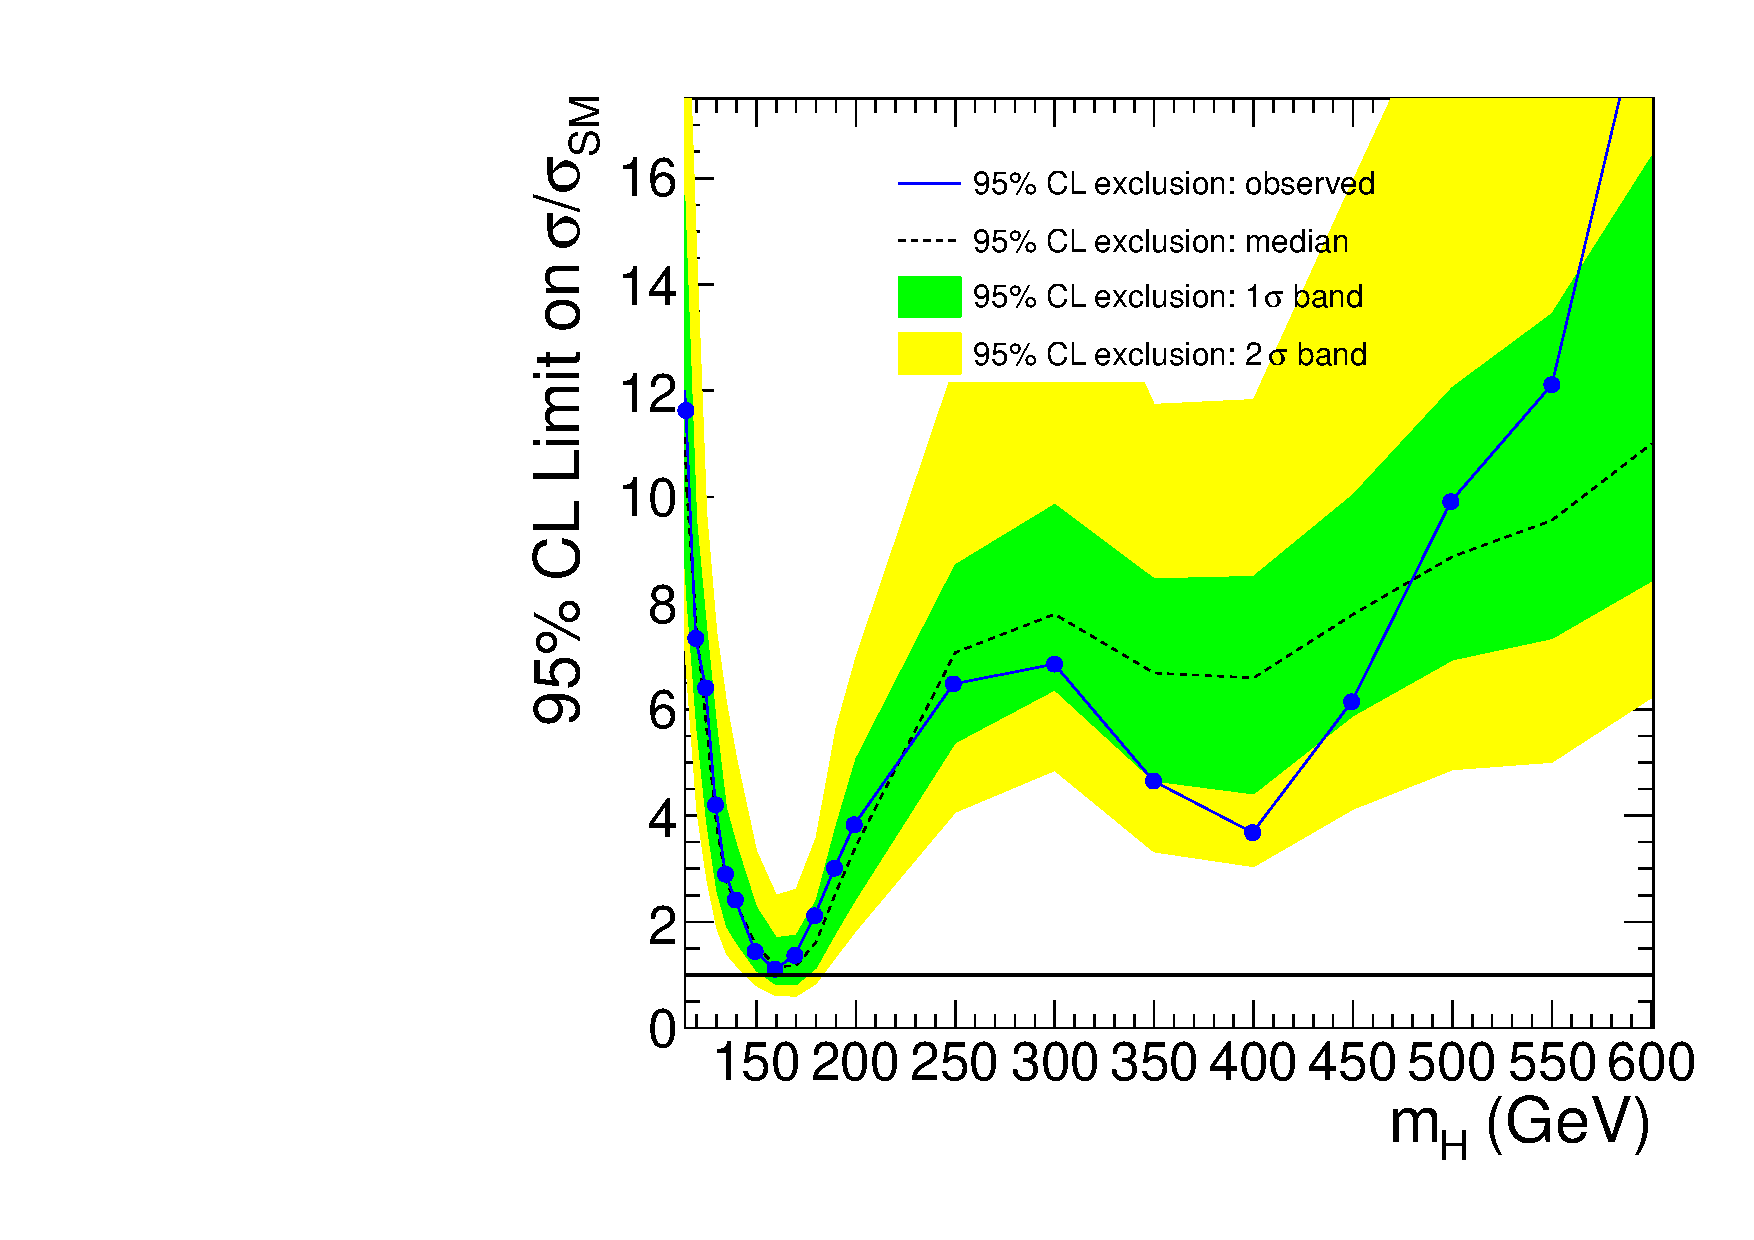
\includegraphics[width=0.49\textwidth]{figures/limits8TeV_ofshape_HCP_2D_BTAG.pdf}
\caption{\label{fig:limits8TeV_ofshapeN_HCP_2D_BTAG}\protect Expected and observed limits for the two-dimensional 
analysis in the 0-jet bin (top left), 1-jet bin (top right), and 0/1-jet bins (bottom), for 
the analysis selecting events in the b-tagged region.}
\end{center}
\end{figure}

\begin{figure}[hbt!]
\begin{center}
  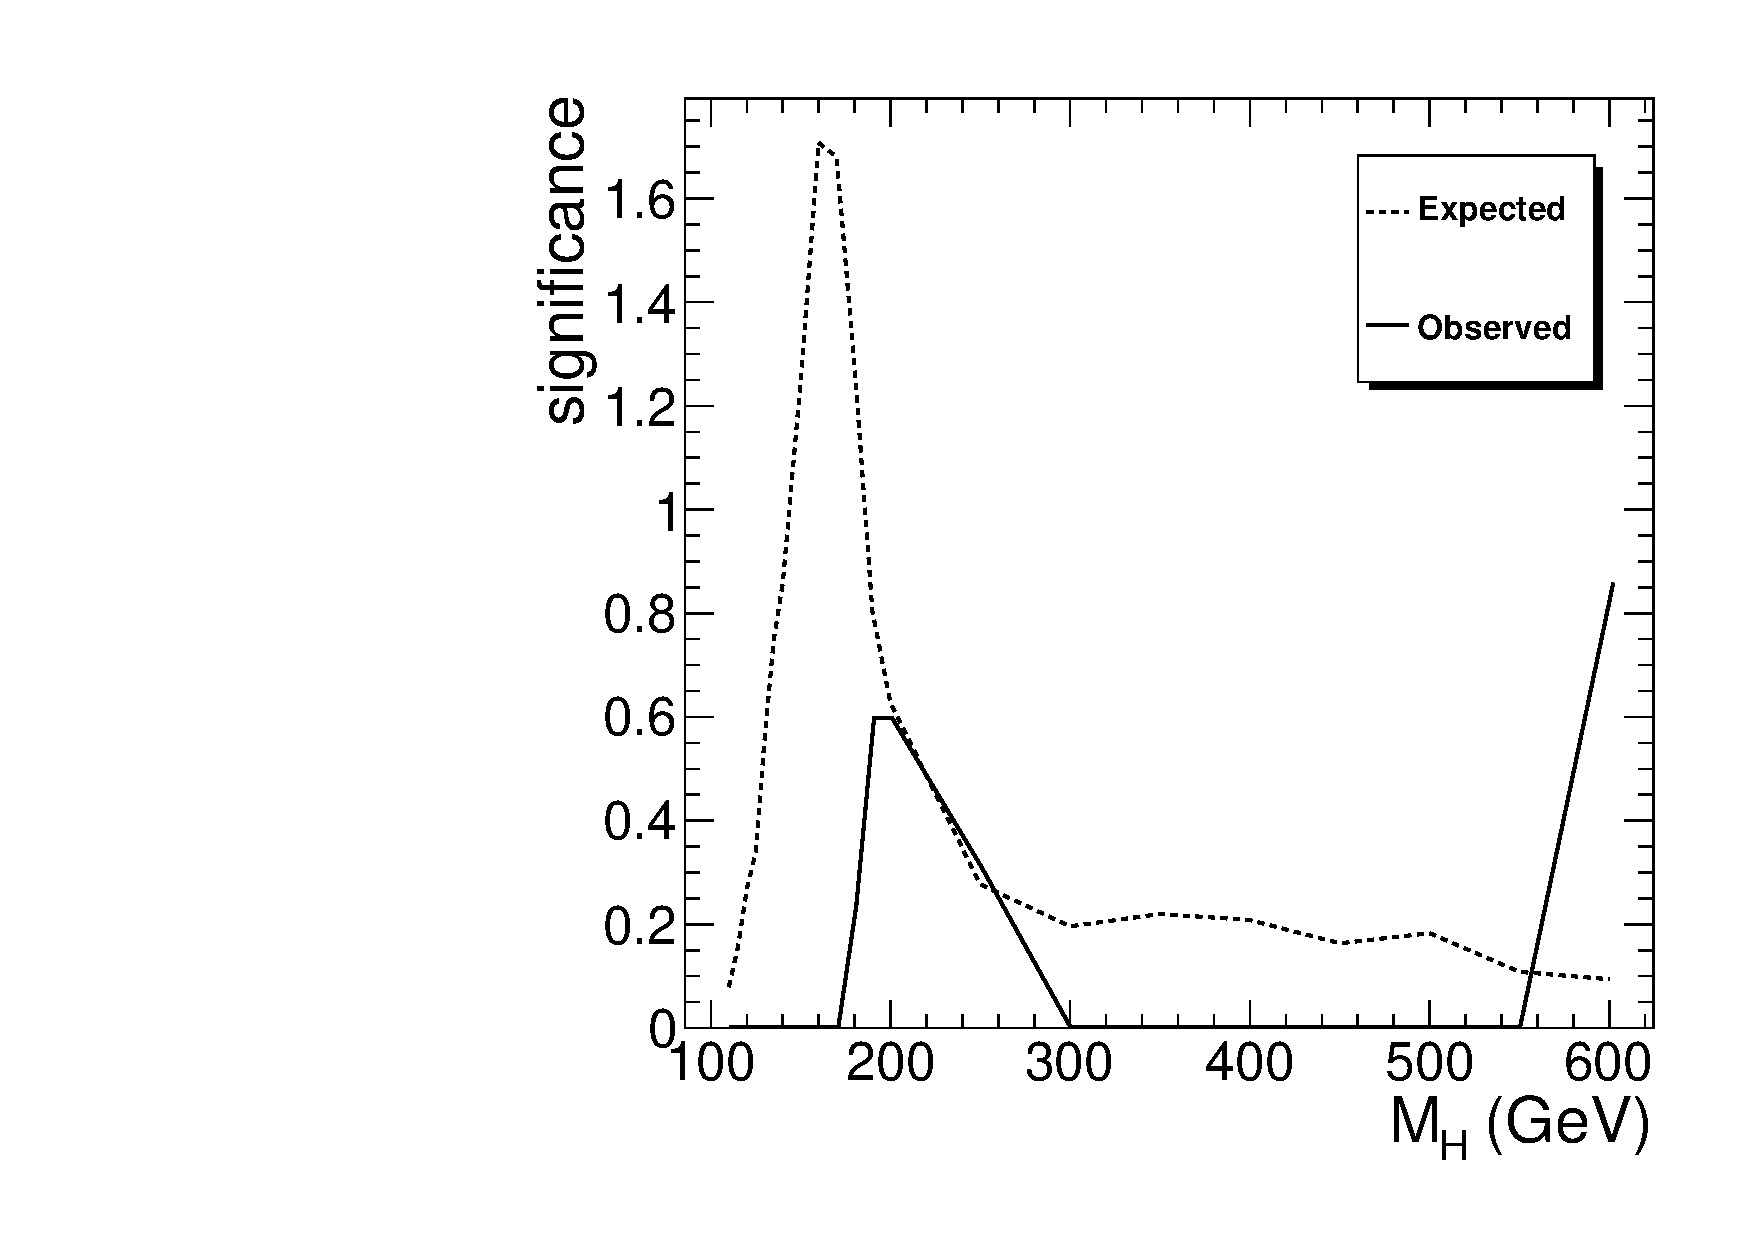
\includegraphics[width=0.49\textwidth]{figures/significance8TeV_ofshape0_HCP_2D_BTAG.pdf}
  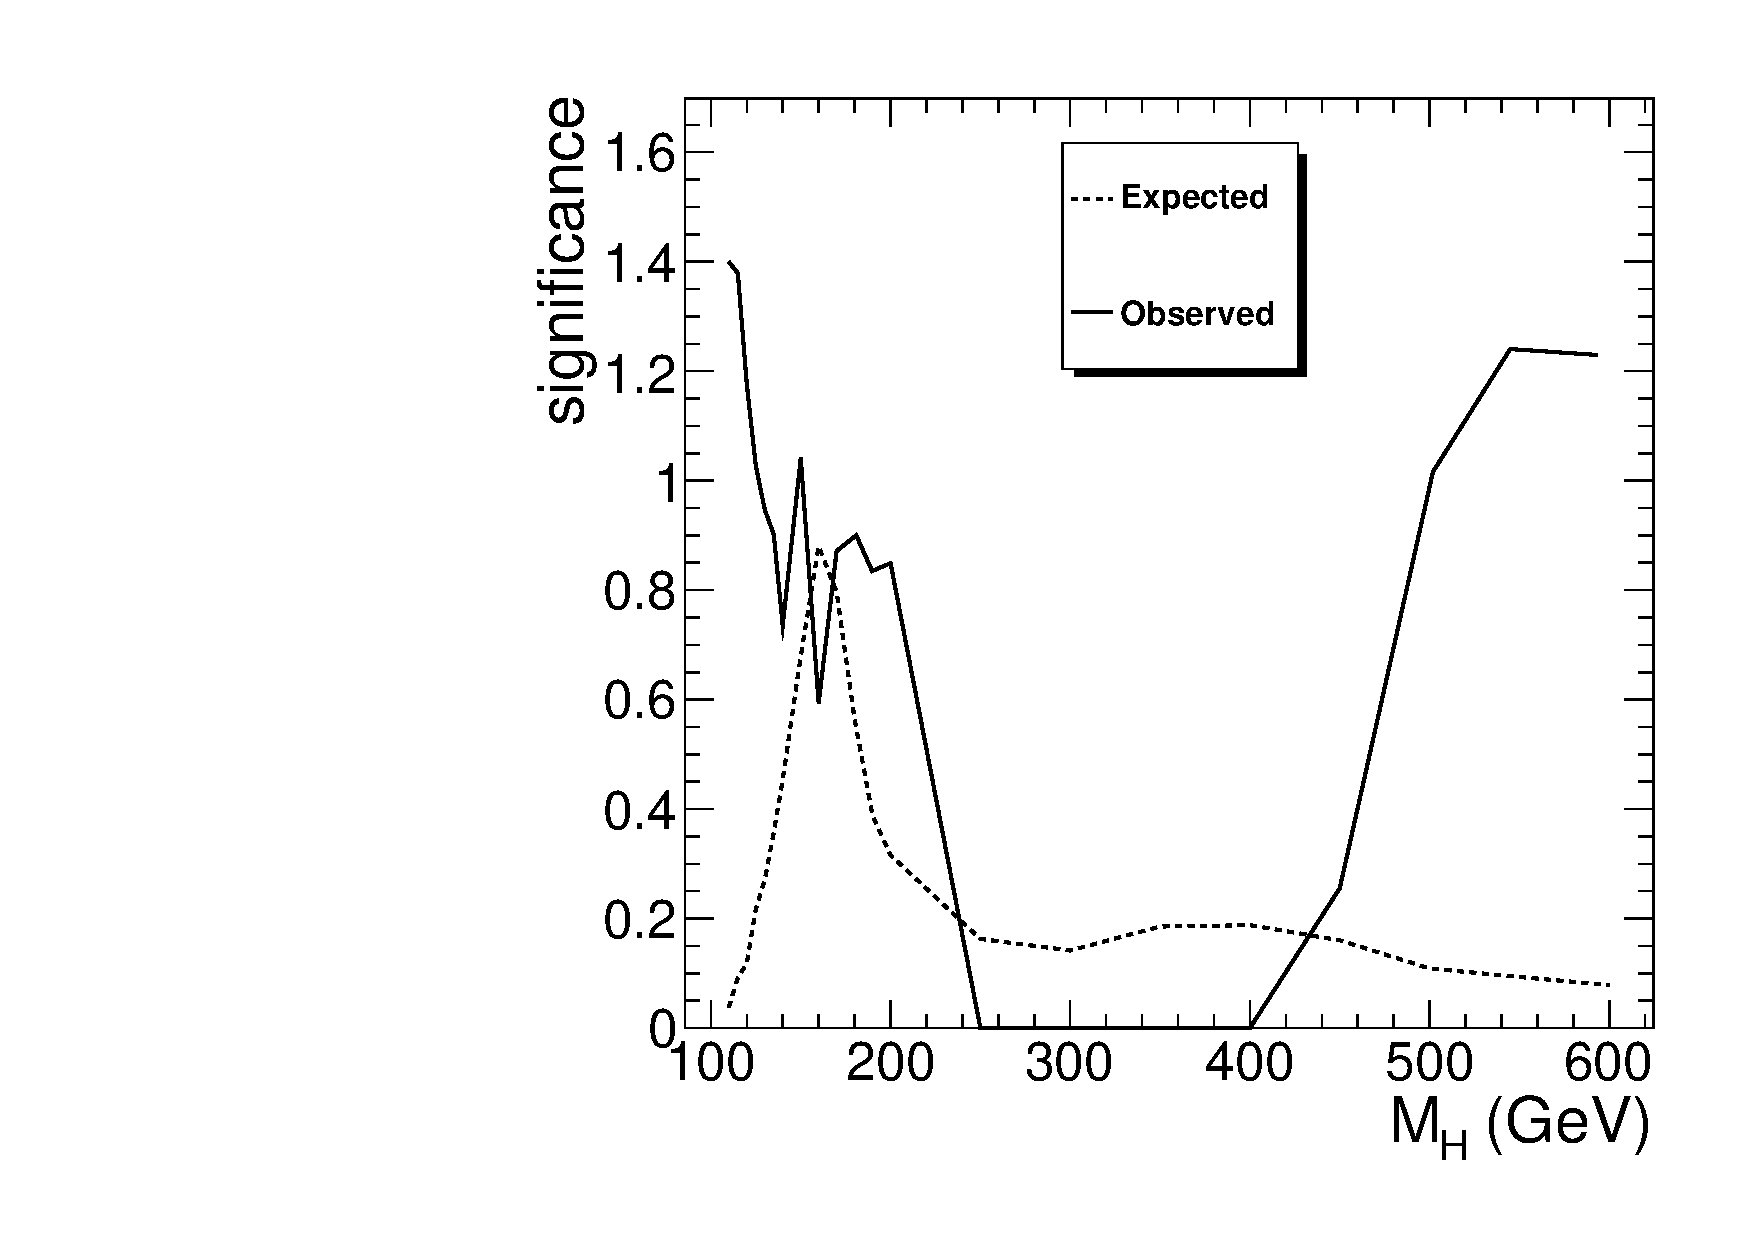
\includegraphics[width=0.49\textwidth]{figures/significance8TeV_ofshape1_HCP_2D_BTAG.pdf}
  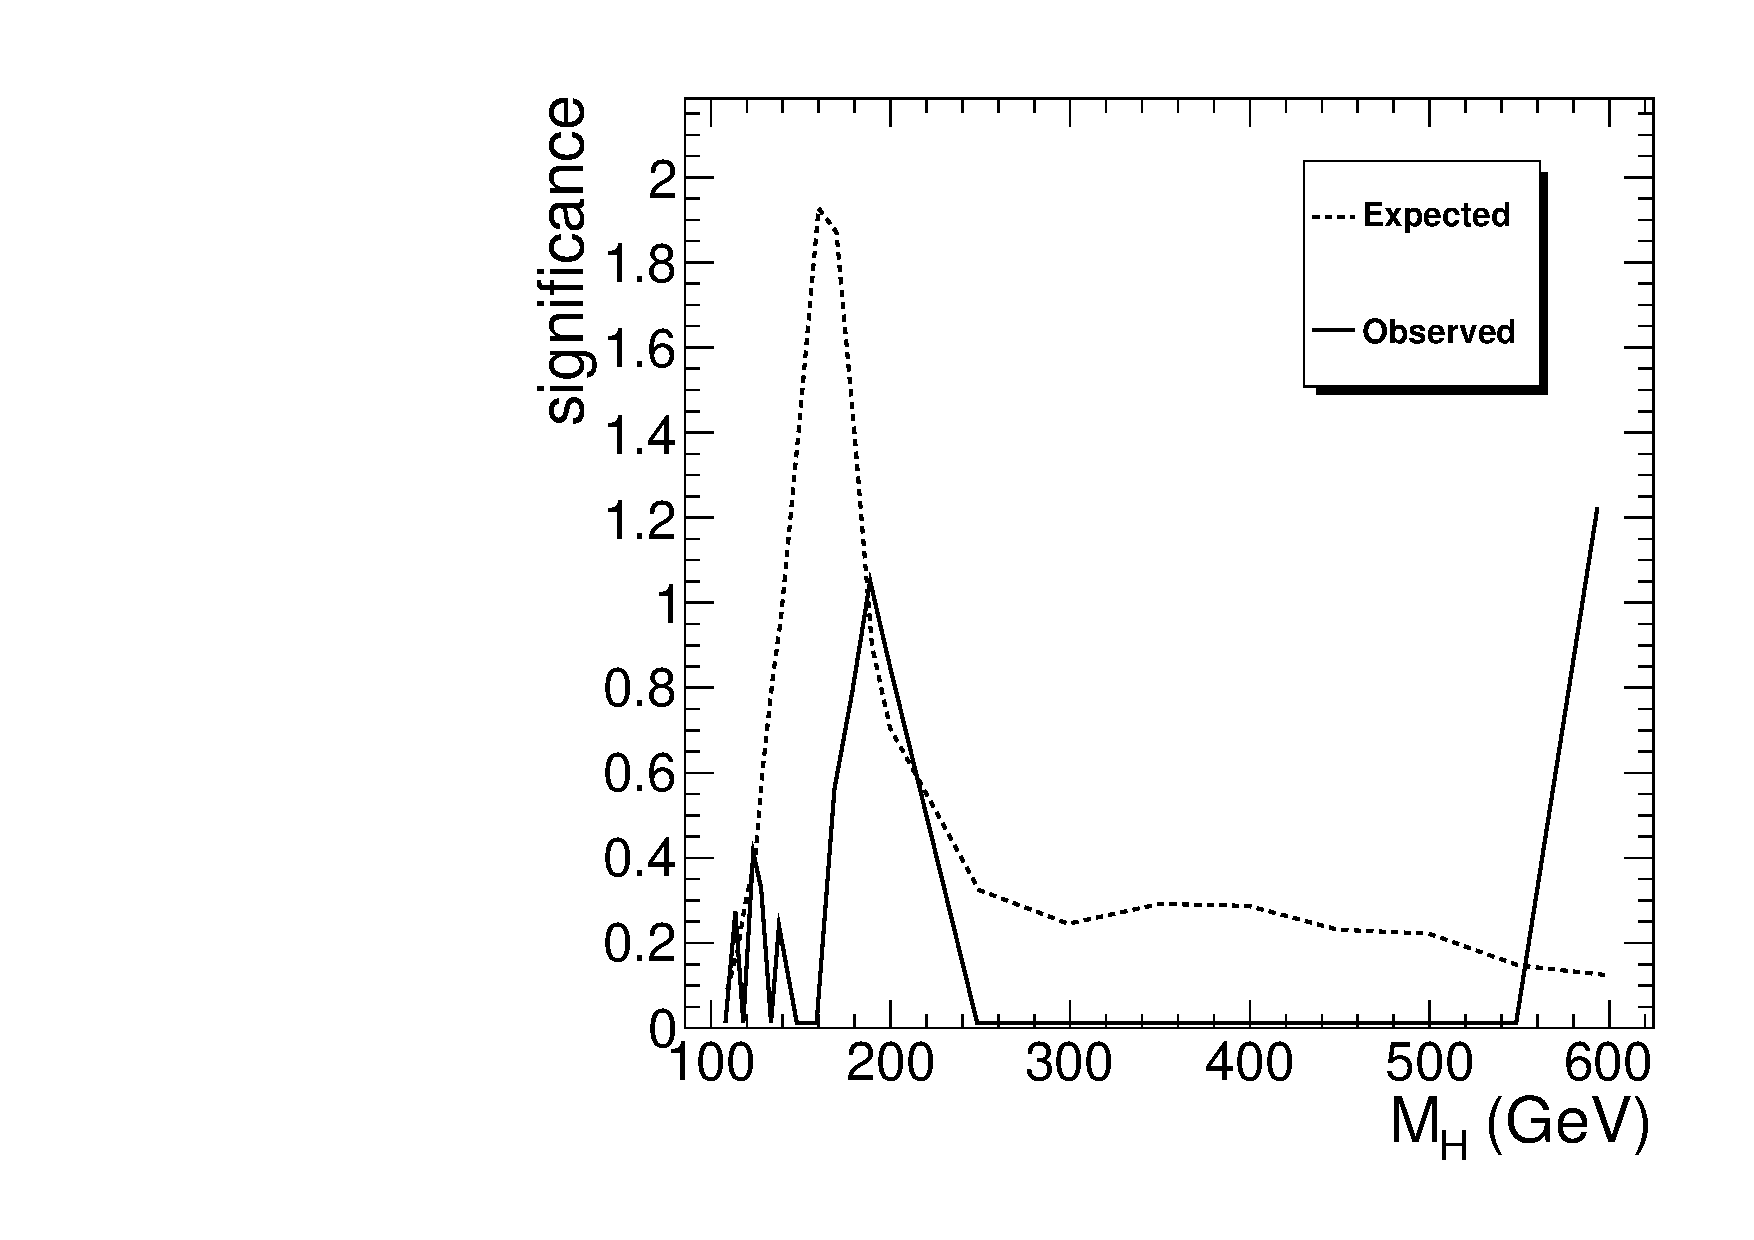
\includegraphics[width=0.49\textwidth]{figures/significance8TeV_ofshape_HCP_2D_BTAG.pdf}
\caption{\label{fig:significance8TeV_ofshapeN_HCP_2D_BTAG}\protect Expected and observed significance for the two-dimensional 
analysis in the 0-jet bin (top left), 1-jet bin (top right), and 0/1-jet bins (bottom), for 
the analysis selecting events in the b-tagged region.}
\end{center}
\end{figure}

\subsection{Same-Sign Lepton Pairs Region}
This analysis selects events with same-sign lepton pairs, i.e. it is enriched in $\Wjets$ and $\W+\gamma^{(*)}$ 
events. The performance of this analysis is extremely small due to the very low rate of Higgs 
events with same-sign lepton pairs. Therefore, it is good enough to show the $\mt$ distributions 
in the data and background prediction, see Fig.~\ref{fig:histo_mt_0j_hw160_ss}, where good agreement 
is observed.

\begin{figure}[hbt!]
\begin{center}
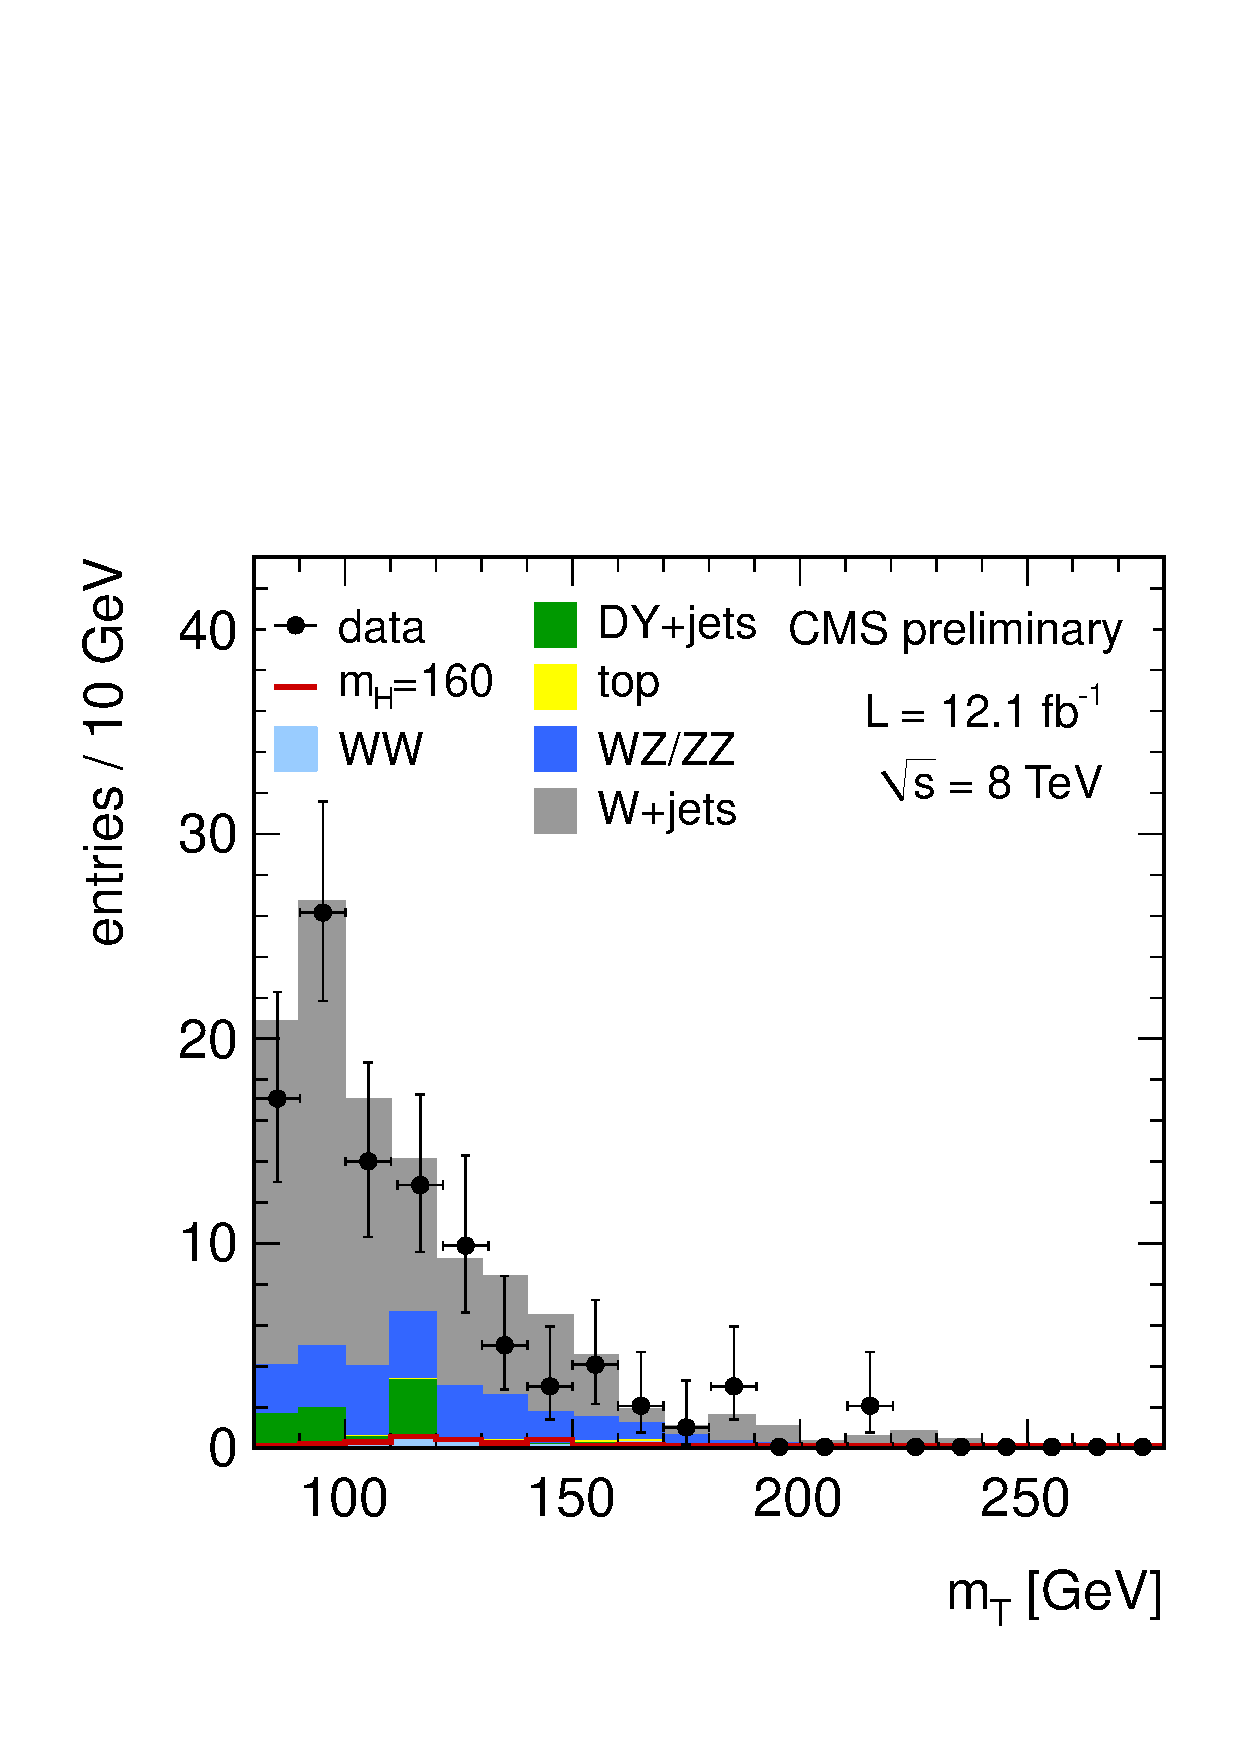
\includegraphics[width=0.49\linewidth]{figures/histo_mt_0j_hw160_ss.pdf}
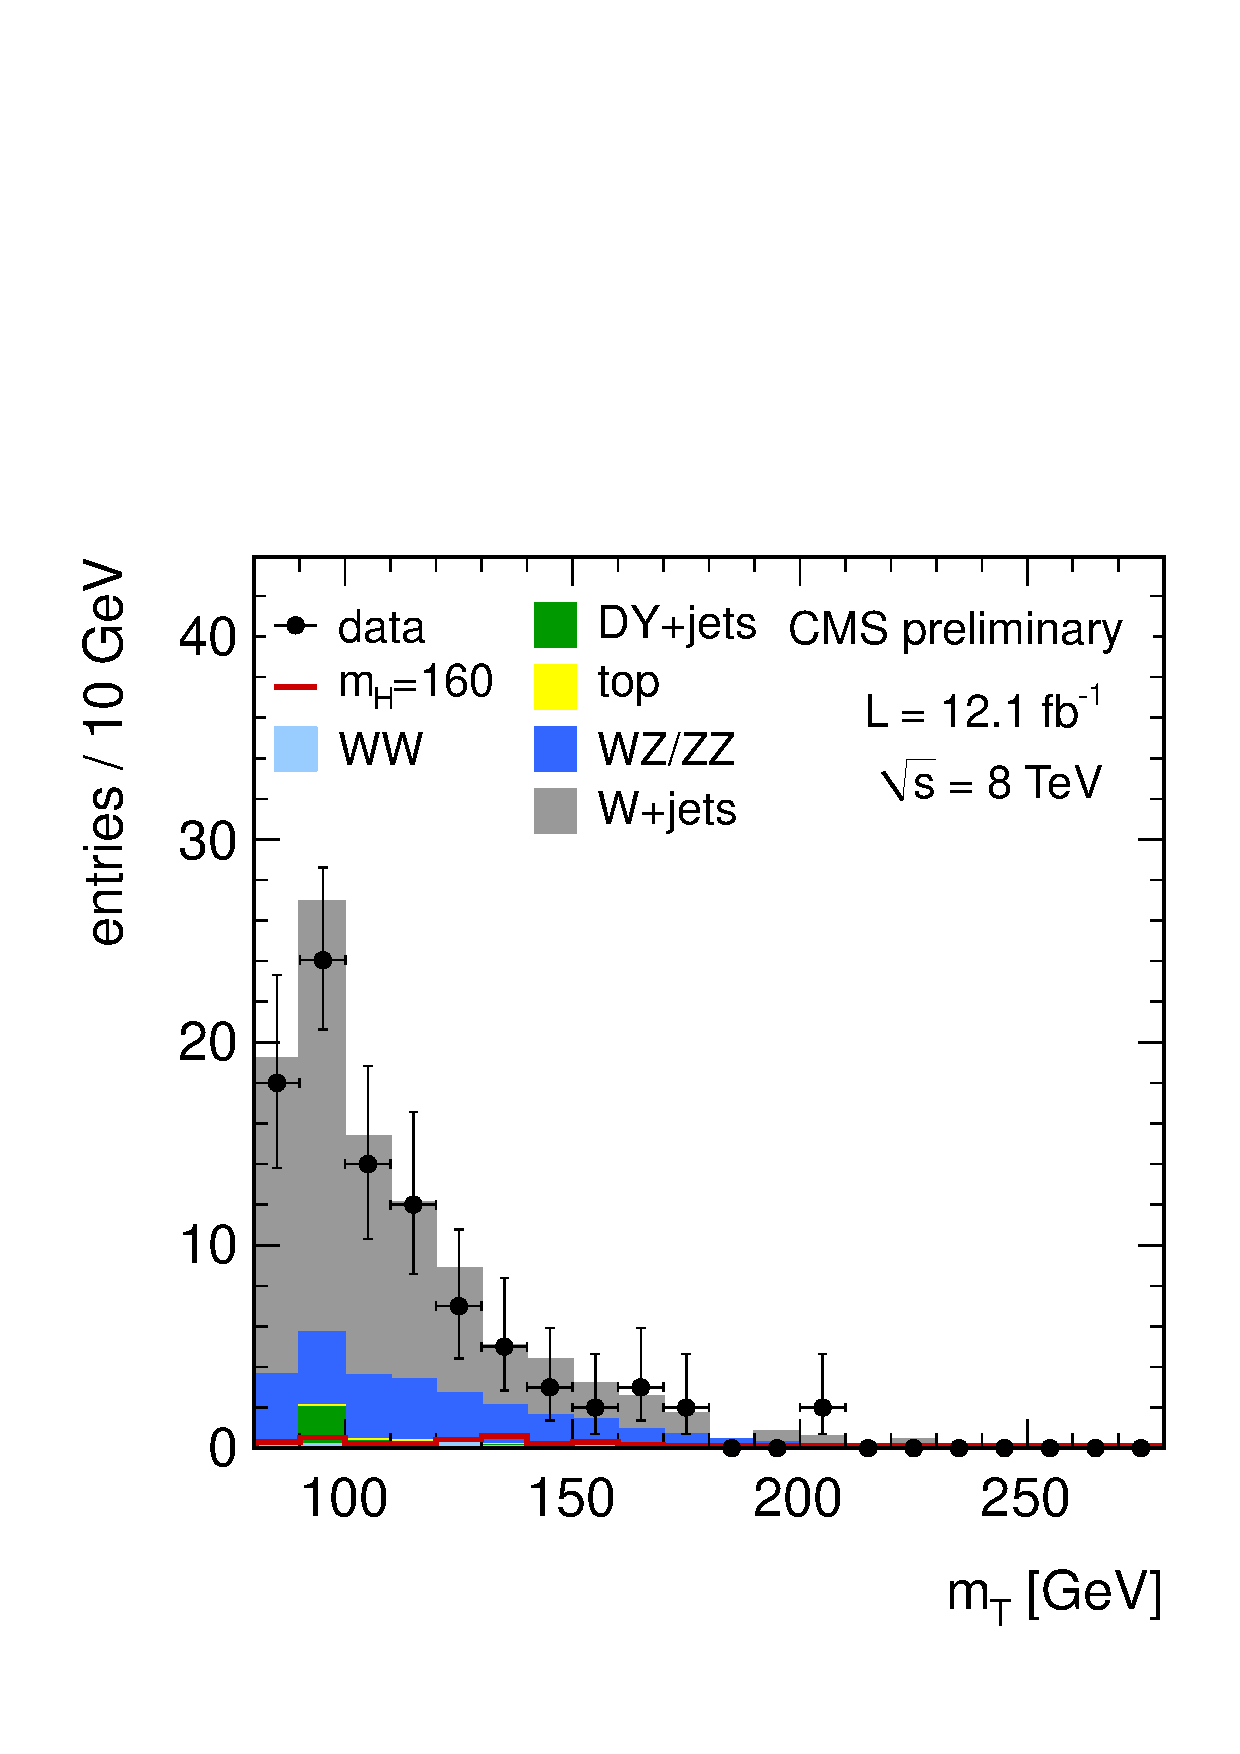
\includegraphics[width=0.49\linewidth]{figures/histo_mt_1j_hw160_ss.pdf}
\caption{\label{fig:histo_mt_0j_hw160_ss}\protect $\mt$ distributions in the 0-jet bin (left) 
and 1-jet bin (right) for events with $\mll<80~\GeV$ in events with same-sign lepton pairs.}
\end{center}
\end{figure}

\subsection{Using H(125) as Additional Component of the Background prediction}
In this analysis the expected yield from $\mHi = 125~\GeV$ is added to the background 
prediction. Including this component in the background will likely make dissapear any excess 
at low Higgs masses, but it is important to see its behavior at higher mass hypotheses. The 
Expected and observed limits for the two-dimensional analysis are shown in 
Fig.~\ref{fig:limits8TeV_ofshapeN_HCP_2D_WithH125_zoom}, while the expected and observed 
significances are shown in Fig.~\ref{fig:significance8TeV_ofshapeN_HCP_2D_WithH125_zoom}.

\begin{figure}[hbt!]
\begin{center}
  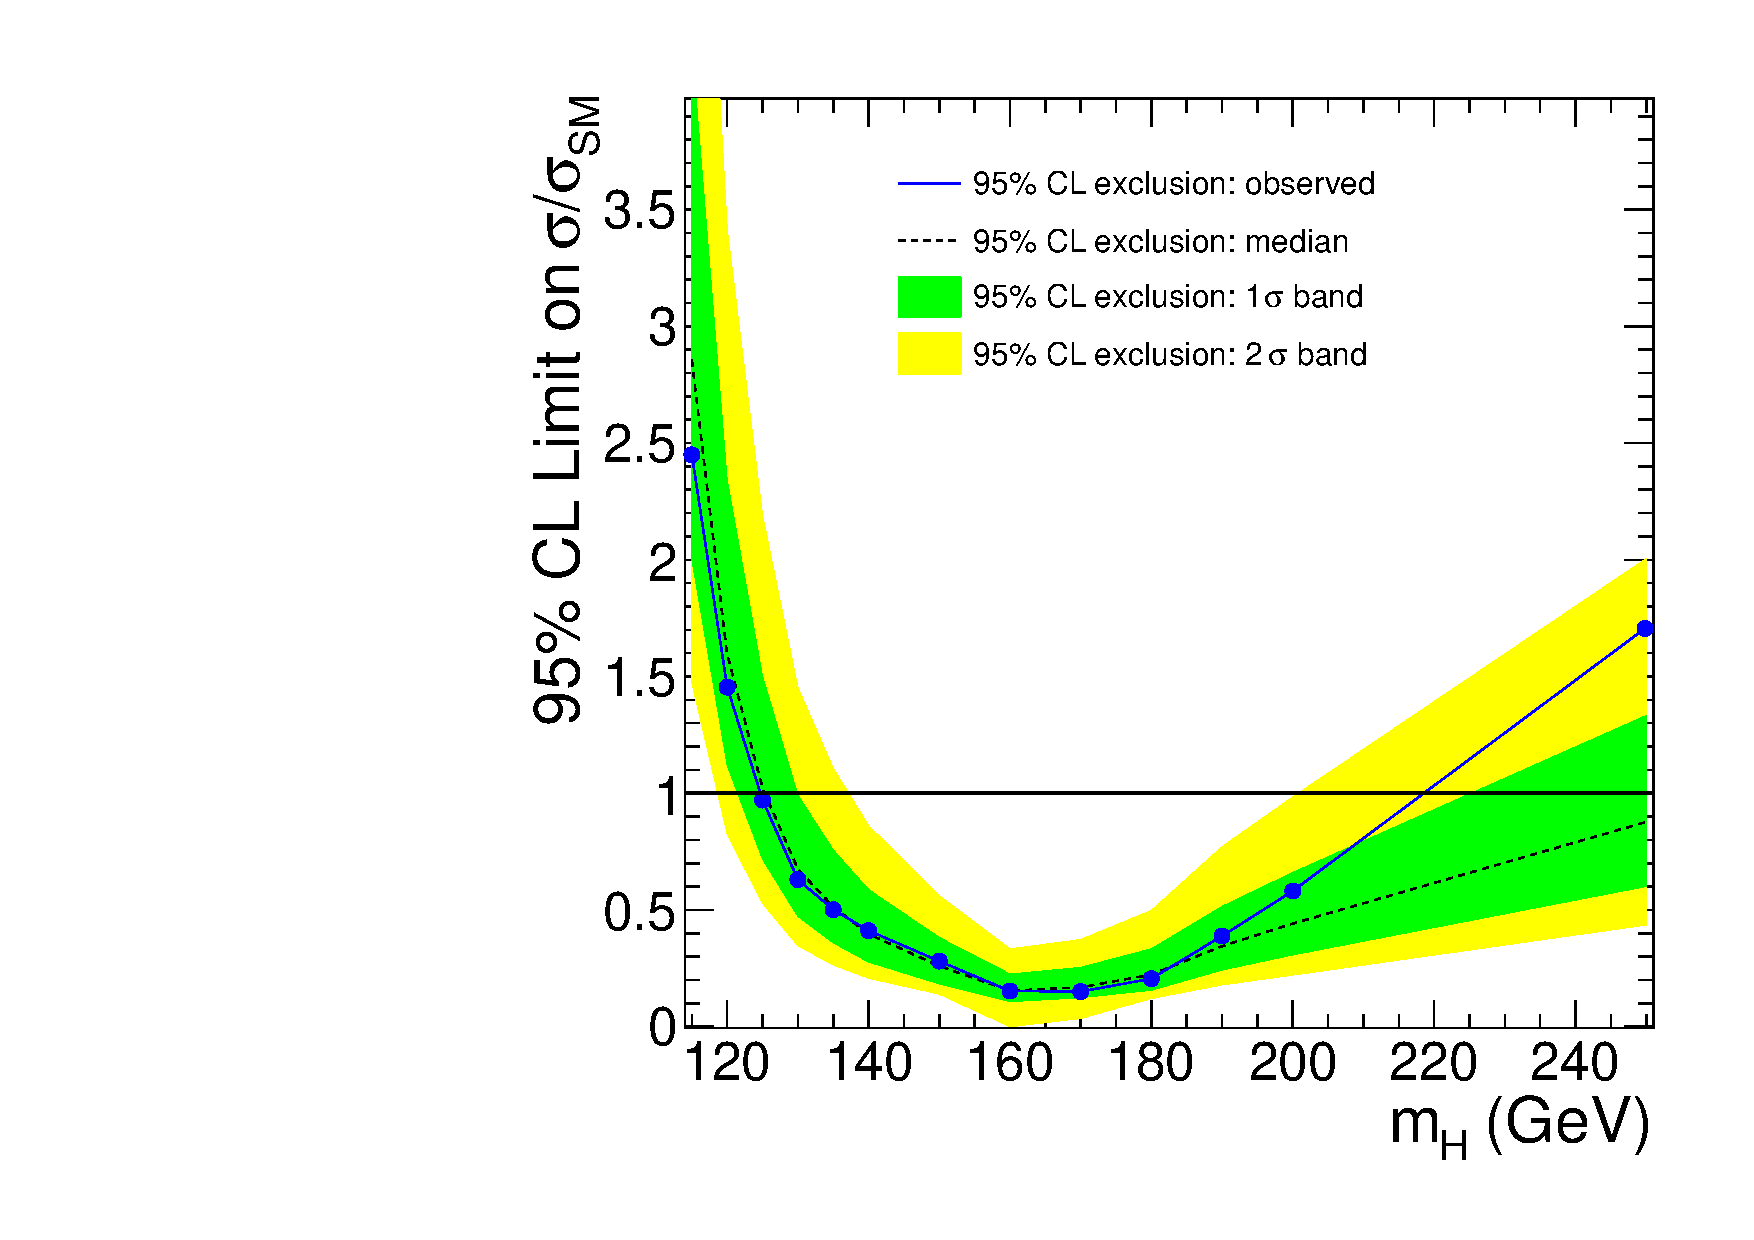
\includegraphics[width=0.49\textwidth]{figures/limits8TeV_ofshape0_HCP_2D_WithH125_zoom.pdf}
  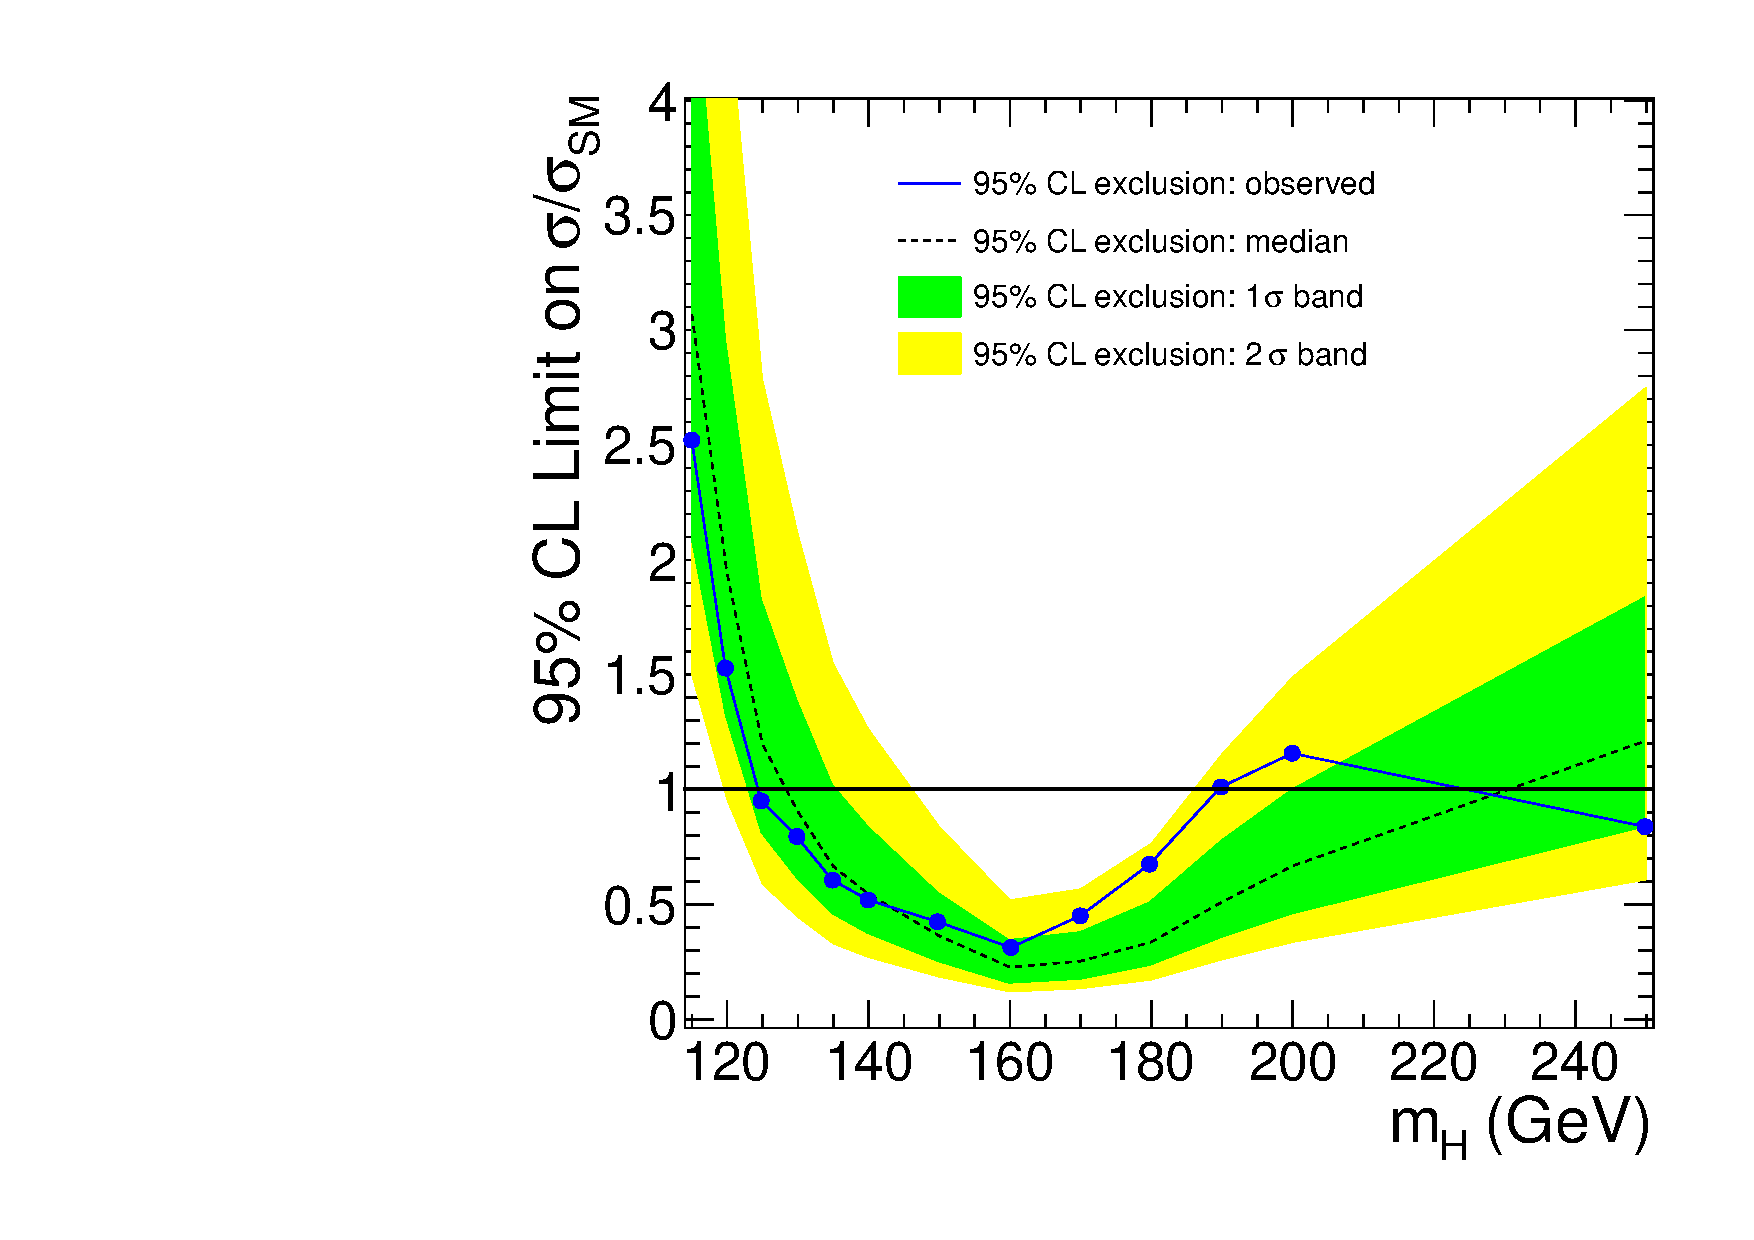
\includegraphics[width=0.49\textwidth]{figures/limits8TeV_ofshape1_HCP_2D_WithH125_zoom.pdf}
  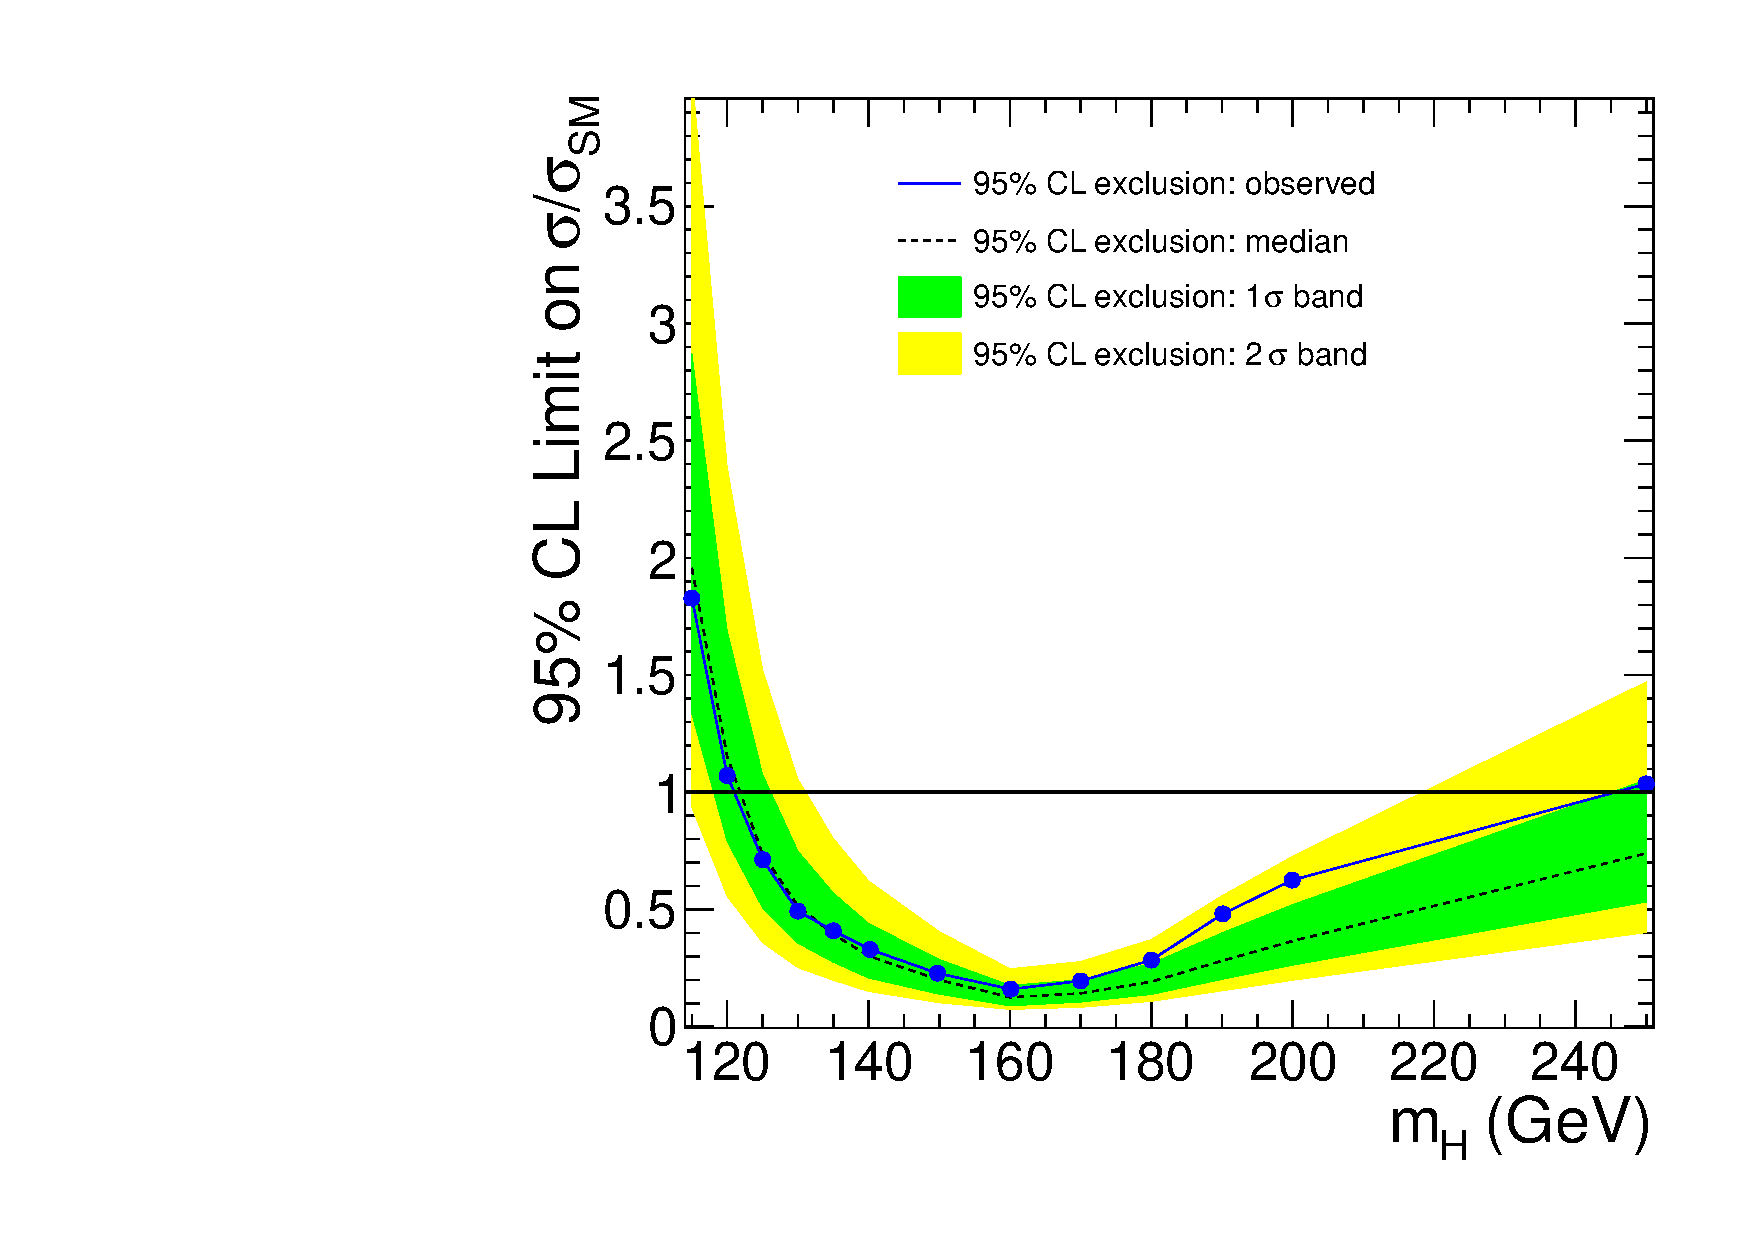
\includegraphics[width=0.49\textwidth]{figures/limits8TeV_ofshape_HCP_2D_WithH125_zoom.pdf}
\caption{\label{fig:limits8TeV_ofshapeN_HCP_2D_WithH125_zoom}\protect Expected and observed limits for the two-dimensional 
analysis in the 0-jet bin (top left), 1-jet bin (top right), and 0/1-jet bins (bottom), for 
the analysis including $\mHi = 125~\GeV$ as part of the background.}
\end{center}
\end{figure}

\begin{figure}[hbt!]
\begin{center}
  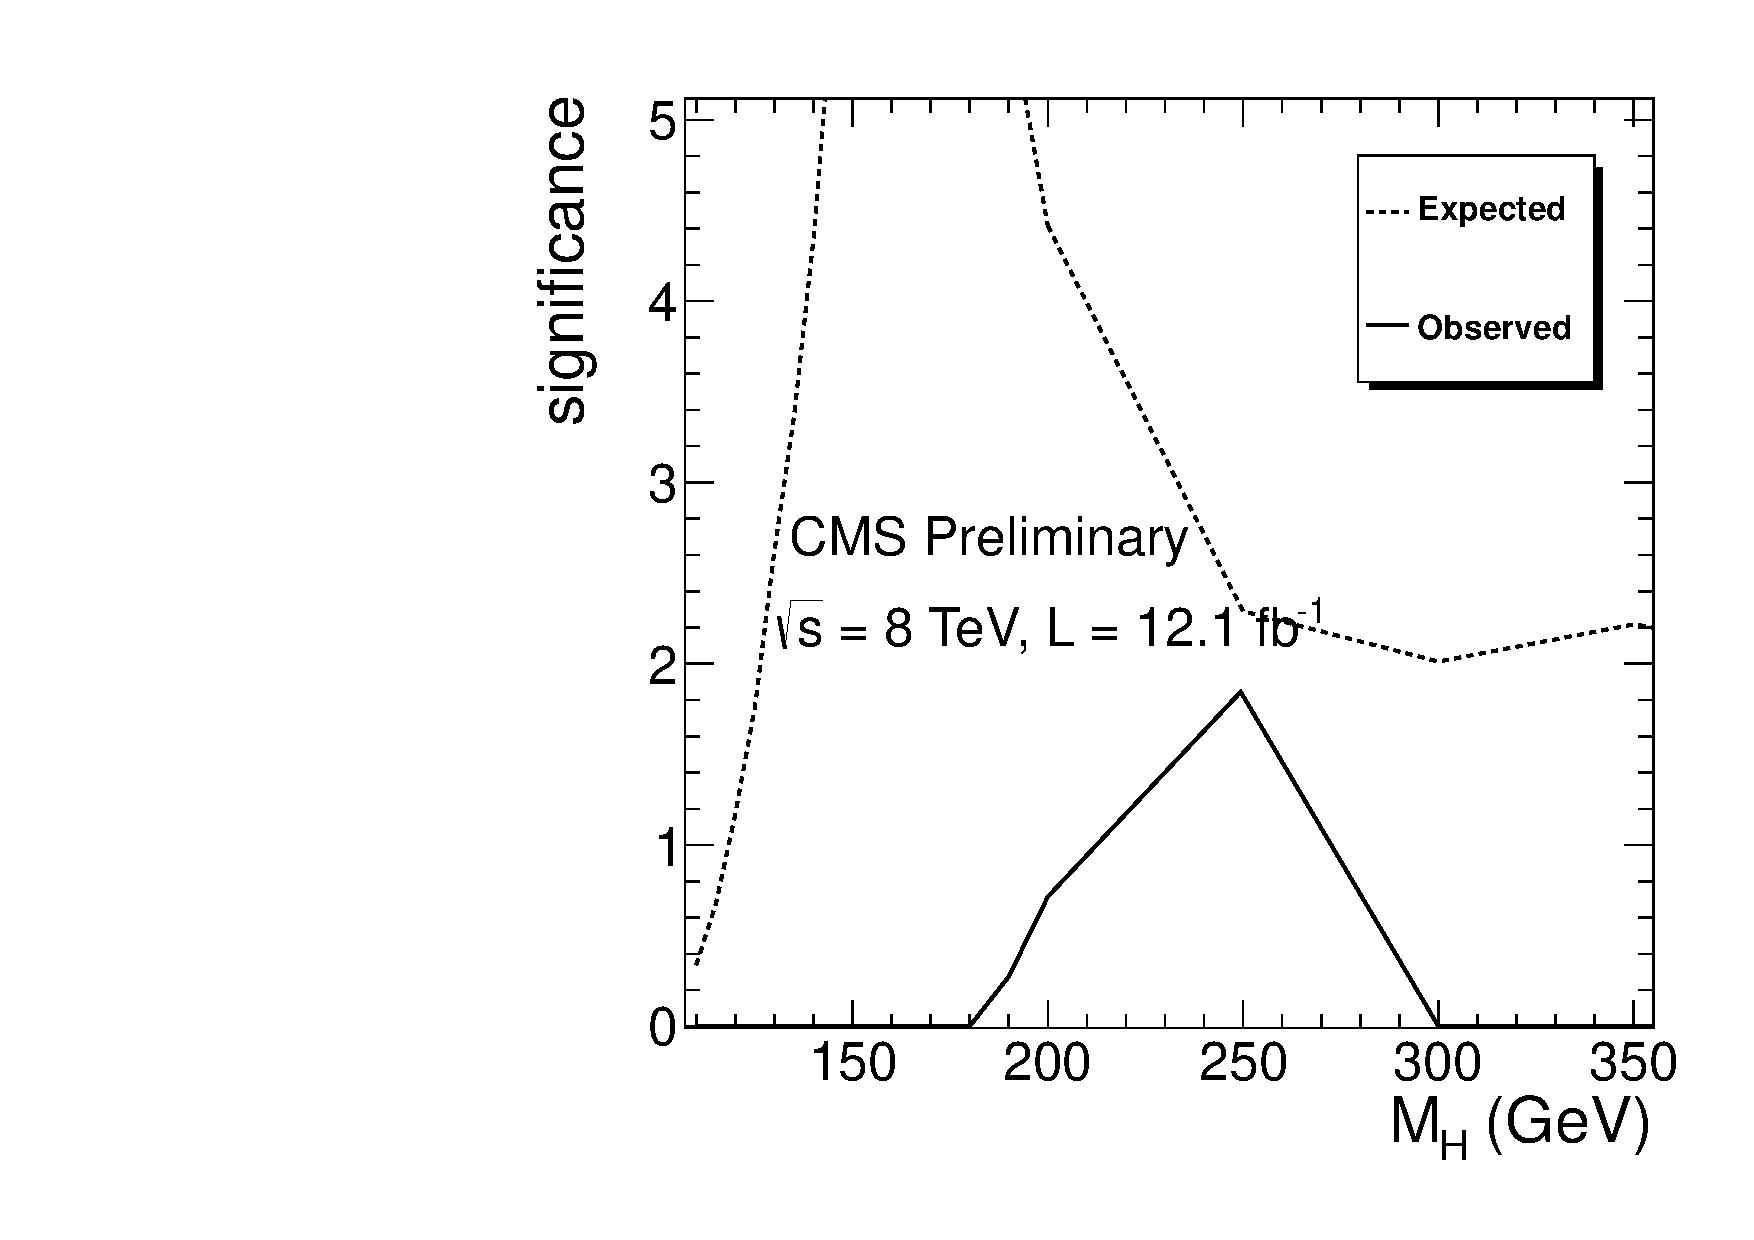
\includegraphics[width=0.49\textwidth]{figures/significance8TeV_ofshape0_HCP_2D_WithH125_zoom.pdf}
  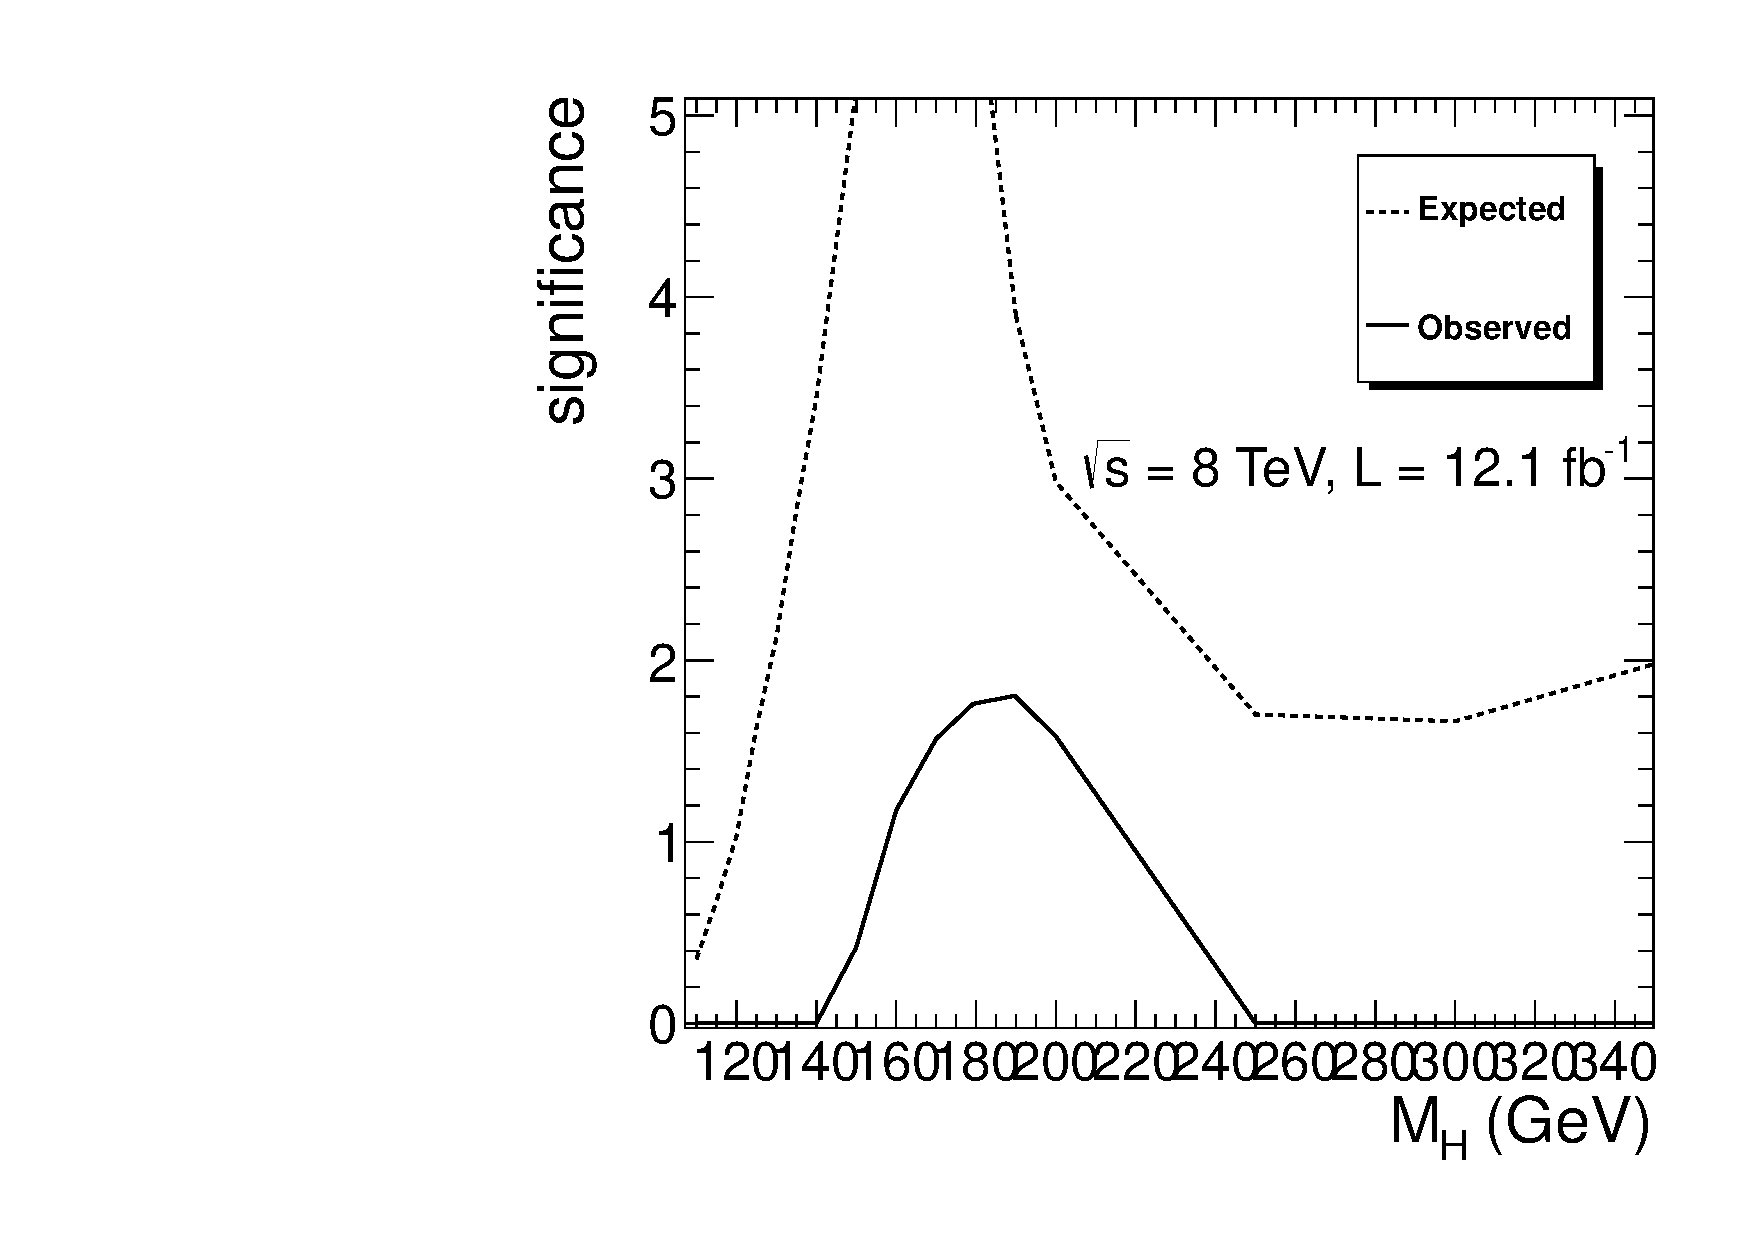
\includegraphics[width=0.49\textwidth]{figures/significance8TeV_ofshape1_HCP_2D_WithH125_zoom.pdf}
  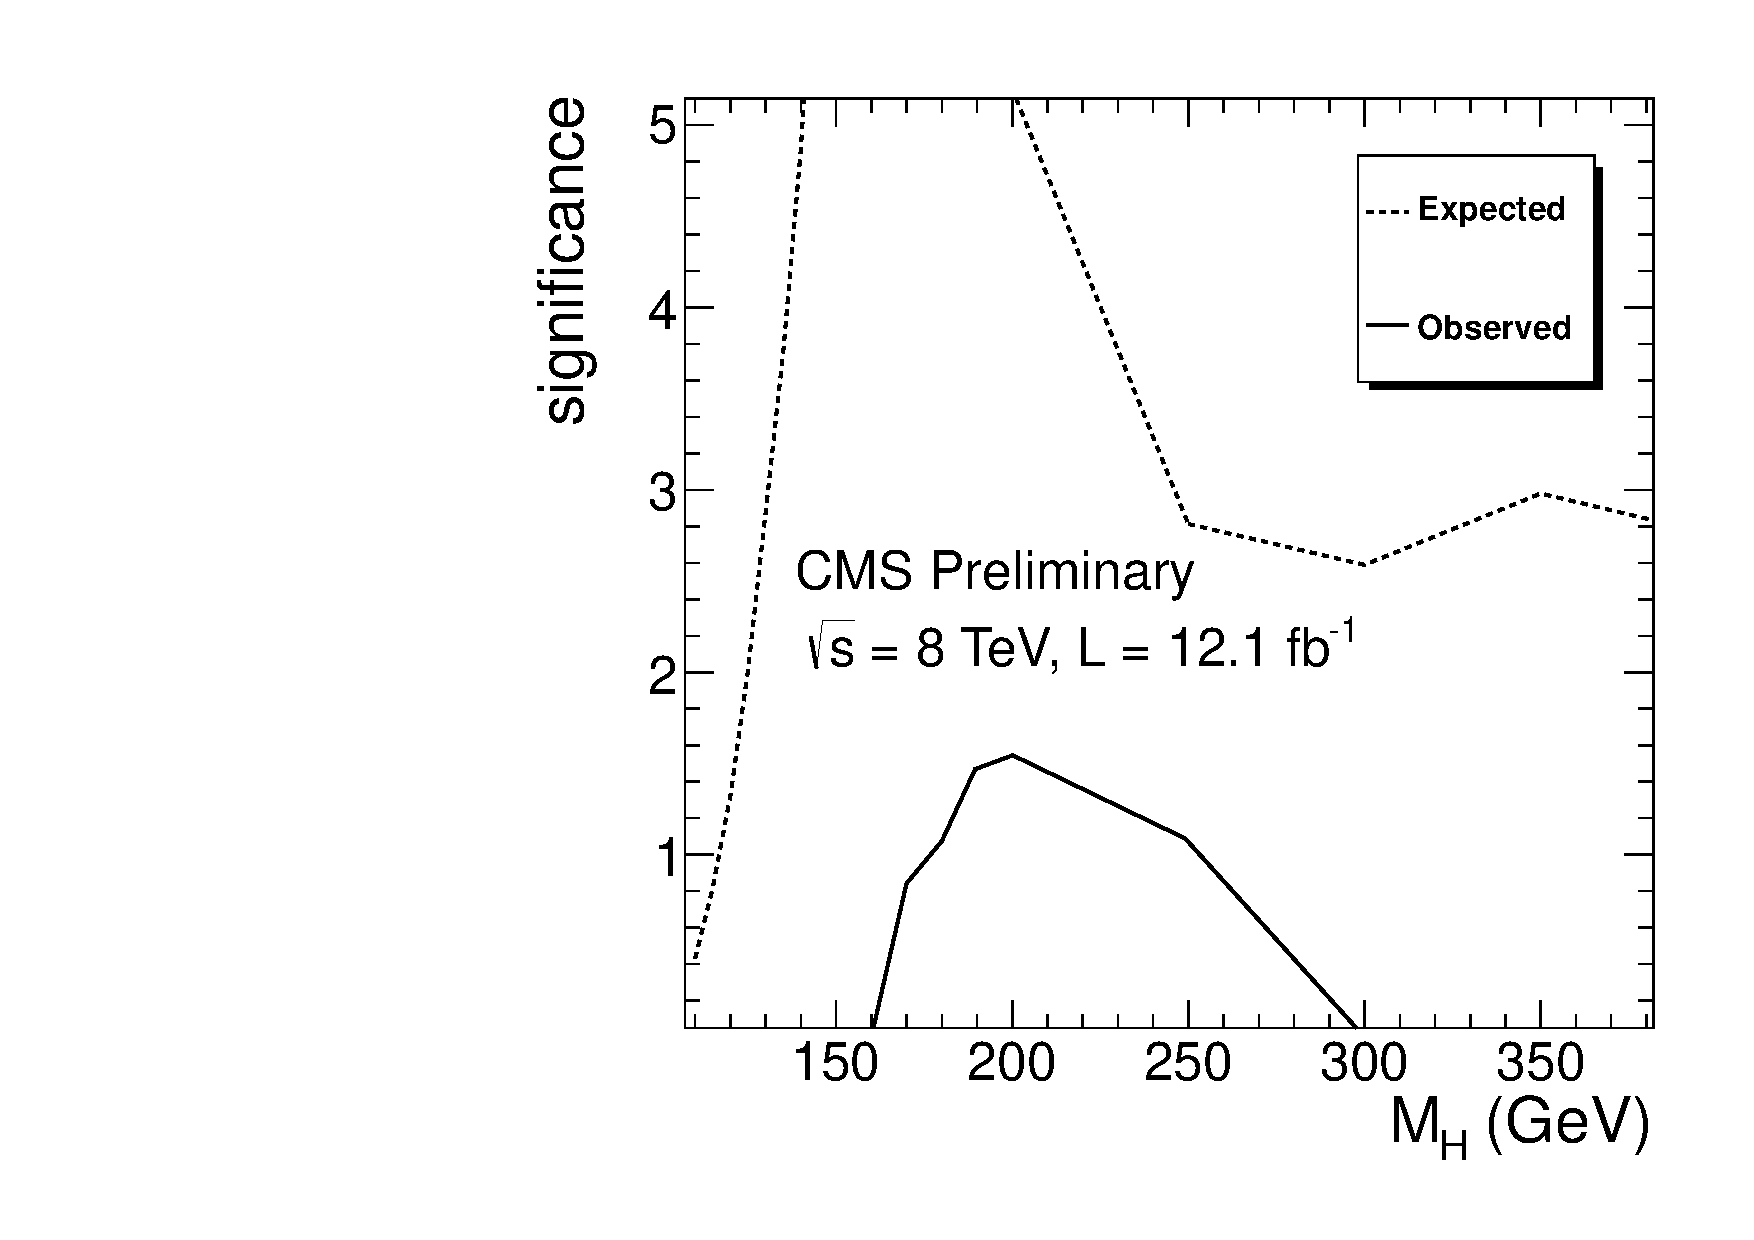
\includegraphics[width=0.49\textwidth]{figures/significance8TeV_ofshape_HCP_2D_WithH125_zoom.pdf}
\caption{\label{fig:significance8TeV_ofshapeN_HCP_2D_WithH125_zoom}\protect Expected and observed significance for the two-dimensional 
analysis in the 0-jet bin (top left), 1-jet bin (top right), and 0/1-jet bins (bottom), for 
the analysis including $\mHi = 125~\GeV$ as part of the background.}
\end{center}
\end{figure}

\subsection{Summary of the Test in Data}
The excess at $m_{T} \sim 130-160~\GeV$ has been investigated by looking at different regions in data, and 
performing the analysis in different ways. All control regions agree reasonable well with the prediction. 
In addition, it is seen that adding H(125) to the background contribution greatly reduce the significance 
of the excess at intermediate Higgs mass hypotheses.
